\documentclass[10pt,a4paper]{article}
\usepackage[ngerman]{babel}
\usepackage[utf8]{inputenc}
\usepackage{xspace}
\usepackage[T1]{fontenc}
\usepackage[pdftex]{graphicx}
\usepackage{listings}
\usepackage{xcolor}
\usepackage{textcomp}

\graphicspath{{./}{./images/}{./chapter/images/}}

\lstset{breaklines=true,
breakatwhitespace = true,
postbreak=\raisebox{0ex}[0ex][0ex]{\ensuremath{\color{red}\hookrightarrow\space}},
escapechar=\^,
basicstyle=\ttfamily
%literate={\_}{}{0\discretionary{\_}{}{\_}}%
}

\title{SQD+KD}
\begin{document}
\maketitle

\section{Anwendungsstart}
\label{sec:startApp}
Beim Start der Anwendung wir als erstes die Konfigurationsdatei durch Aufruf der Methode \lstinline|loadConfigFile()| der Klasse \lstinline|ConfigurationManager| eingelesen. Hierbei wird eine Datei mit dem vordefinierten Namen \lstinline|concierge.conf| verwendet, welche im gleichen Verzeichnis wie die Anwendung liegen muss. Die eingelesenen Werte werden hierbei durch die statische Klasse \lstinline|Constants.Config| verwaltet. Im Anschluss wird eine \lstinline|Application| erzeugt. Der \lstinline|ConciergeController| startet durch Aufruf der Methode \lstinline|menu()| die Ausgabe des Menüs auf der Konsole, sowie die Routine zur Eingabe eines Zahlenwertes, welcher jeweils einer eigenen Funktion entspricht, die im Folgenden aufgerufen wird. Alle Funktionalitäten werden von der Klasse \lstinline|BasicBehaviour| verwaltet. Nachfolgende Möglichkeiten bietet das Menü und deckt die möglichen Eingabewerte von 0-10 ab:

\begin{itemize}
\item 0) Fortlaufende Tour ab ... starten: (true/false)
\item 1) Komplette Tour starten
\item 2) Begrüßung und allgemeine Informationen starten
\item 3) TV Raum starten
\item 4) Arbeitszimmer starten
\item 5) Bad starten
\item 6) Küche starten
\item 7) Verabschiedung starten
\item 8) Smart Home Labor auf Ausgangseinstellungen setzen
\item 9) Reboot Pepper
\item 10) Shutdown Pepper
\end{itemize}

Durch die Eingabe der Zahl 0 kann bestimmt werden, ob ab dem Start eines Raumes, wie zum Beispiel des TV Raumes alle fortfolgenden Räume ebenfalls durchlaufen werden sollen (true), oder nur der jeweilige Raum (false). Alle weiteren Funktionalitäten sind selbsterklärend. 

\begin{figure}[ht]
	\centering
	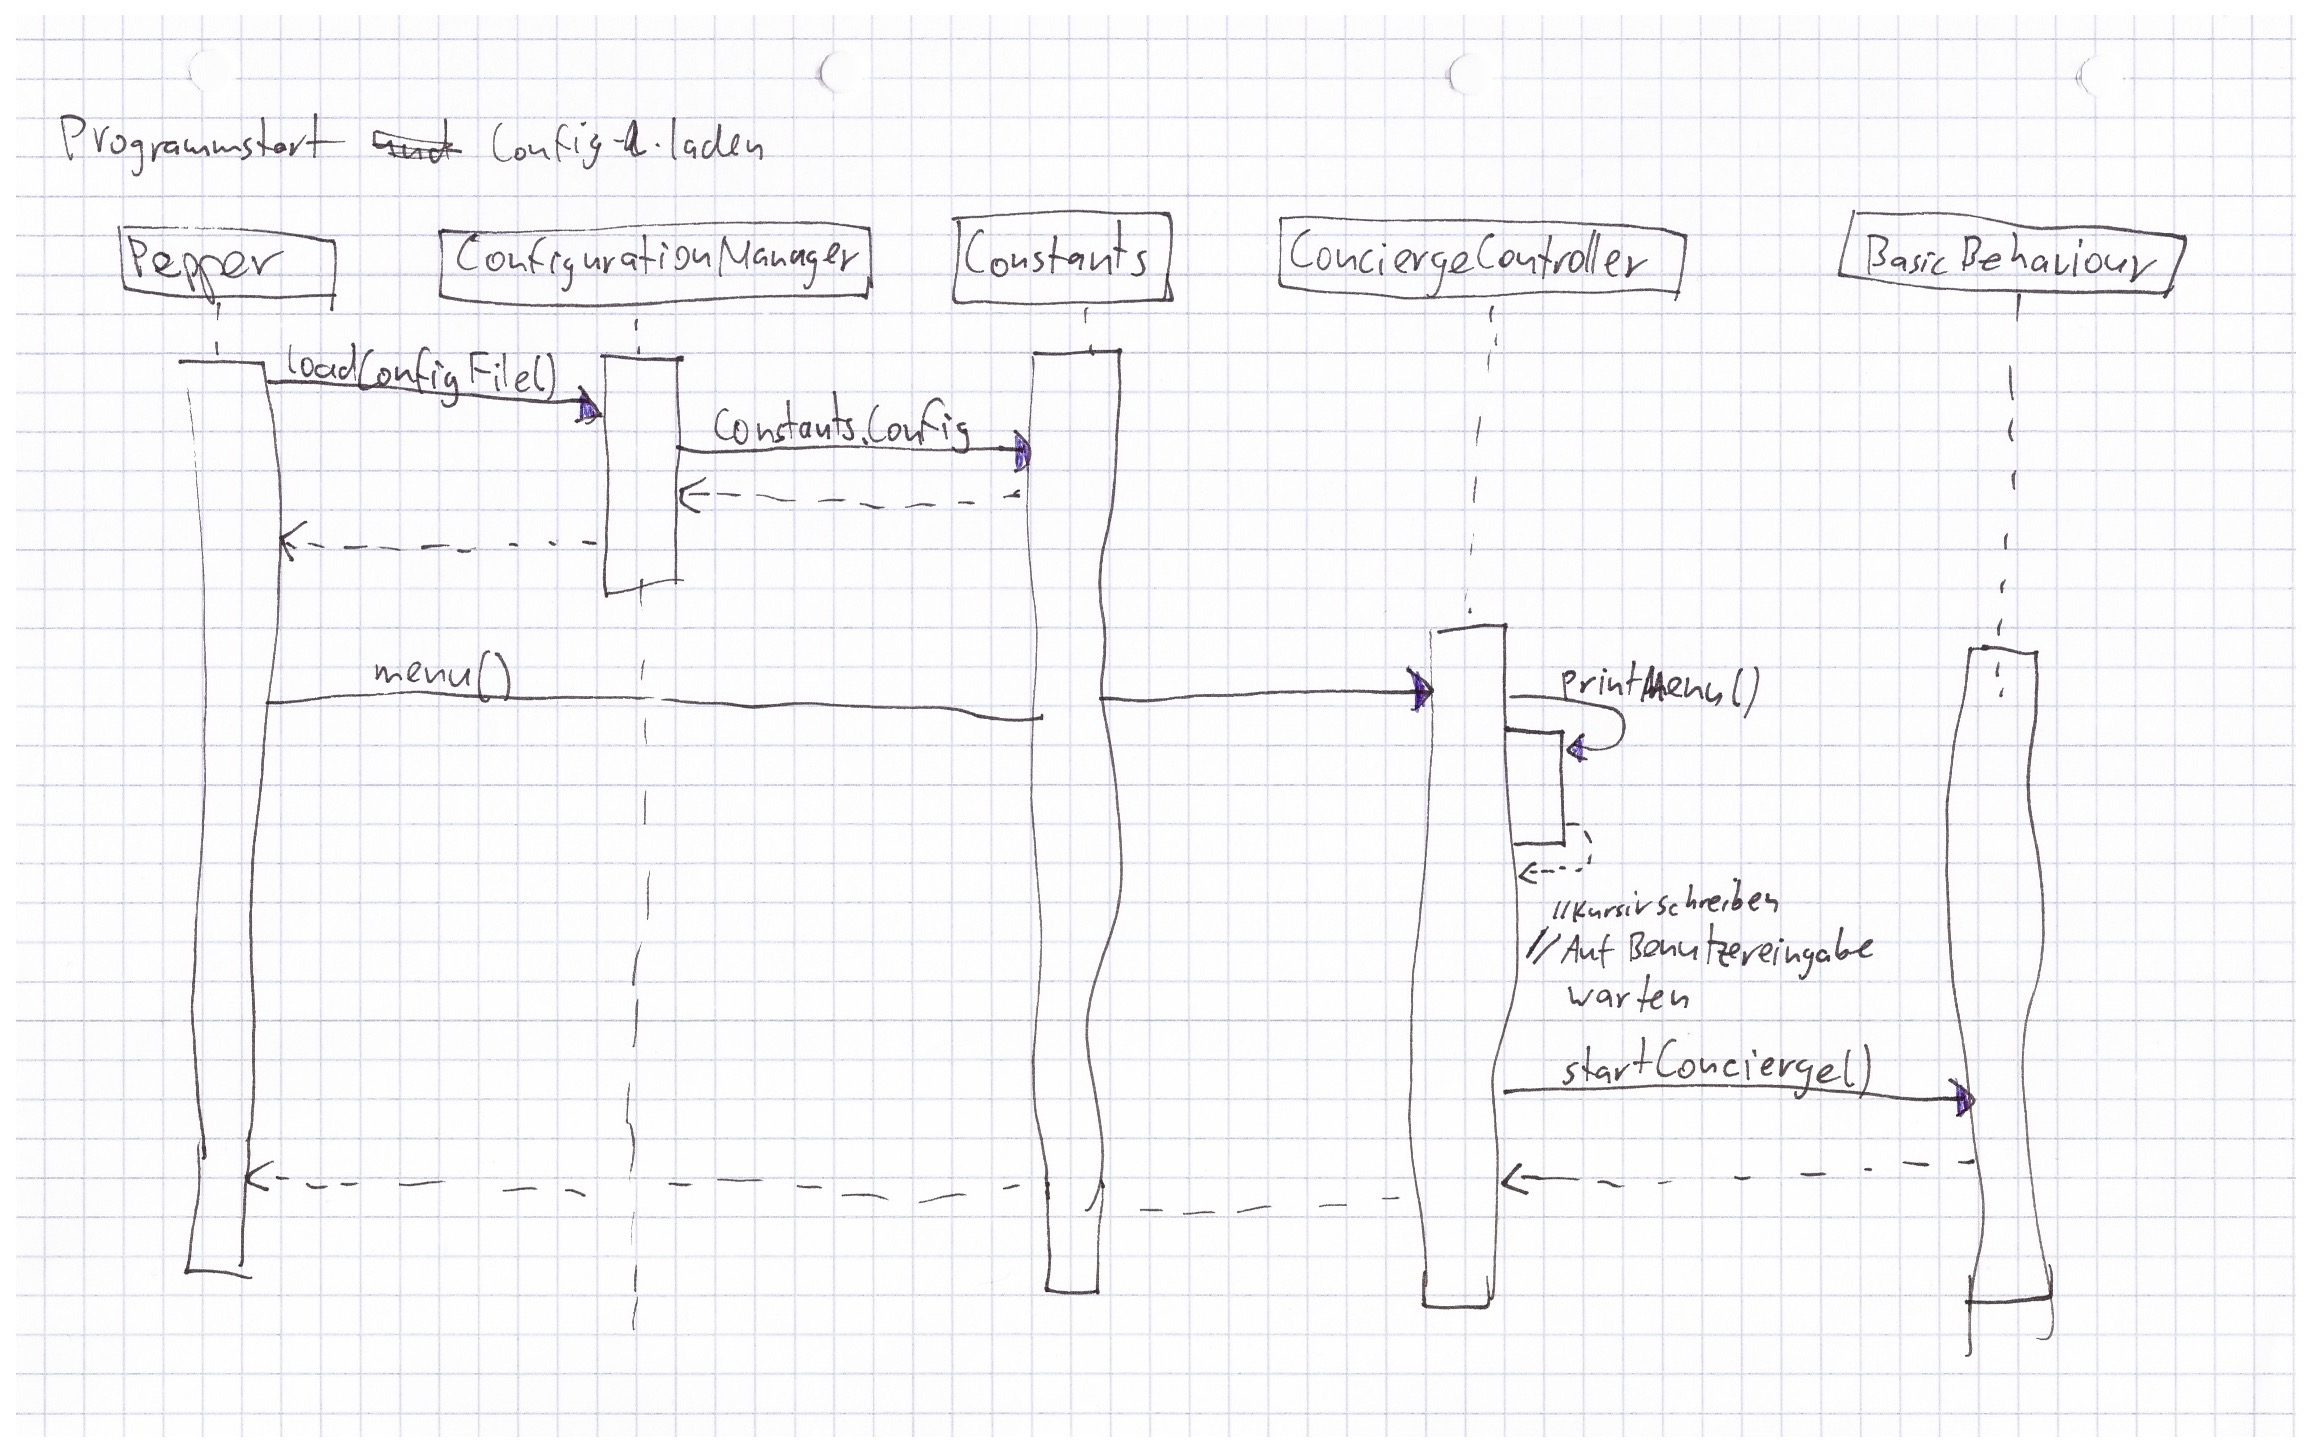
\includegraphics[width=\textwidth]{Scan.jpeg}
	\caption{Sequenzdiagramm - Programmstart und laden der Konfigurationsdatei}
	\label{fig:sqd:appstart}
\end{figure}

\subsection{Aufbau der Konfigurationsdatei}
\label{subsec:configFile}
Die Konfigurationsdatei ist im JSON-Format und beinhaltet folgende Attribute:
\begin{lstlisting}
{
   "pepperIP": "192.168.0.71",
   "headless": false,
   "debug": false,
   "movieUrl": "http://192.168.0.65/video.php?path=videos/CUTRace_v4.mp4",
   "sonosIP": "192.168.0.30",
   "ratingUrl": "http://192.168.0.65/"
}
\end{lstlisting}

Der Wert des Schlüssels \lstinline|pepperIP| gibt die IP-Adresse des jeweiligen Roboters an, welcher zum Ausführen der Anwendung verwendet werden soll. Der Schlüssel \lstinline|headless| gibt an, ob der Rechner, auf welchem die Anwendung ausgeführt und damit der Roboter gesteuert wird, ein Display, sowie Eingabemöglichkeiten besitzt oder nicht. Wird der Wert auf \lstinline|true| gesetzt, so wird davon ausgegangen, dass der Rechner kein 
Display besitzt und somit wird auch kein Menü auf der Konsole ausgegeben. Damit ist es auch nur möglich, die komplette Tour durch das Smart Home Labor durch berühren des Kopfes des Roboters zu starten. Bei aktiviertem \lstinline|Debug|-Modus (\lstinline|debug: true|) werden entsprechende Debug-Meldungen ausgegeben und eine Log-Datei wird erstellt. Der Wert des Schlüssels \lstinline|movieUrl| gibt an, welches Video während der Spieleszene im TV Raum (siehe Abschnitt \ref{subsec:tvRoom}) auf dem Fernseher wiedergegeben werden soll. \lstinline|sonosIP| gibt die IP-Adresse der Sonos-Soundanlage an, auf welcher die Wiedergabe von Musik erfolgen soll. Der letzte Schlüssel \lstinline|ratingUrl| gibt an, wo die Webseite für die Bewertung am Ende der Tour liegt, welche auf Peppers Tablet angezeigt wird (siehe Abschnitt \ref{subsec:goodby}). 
Kann keine Konfigurationsdatei im Verzeichnis gefunden werden, so werden die oben genannten Standardwerte verwendet.  

\section{Initialisierung der Klassen mit Standardwerten}
\label{sec:initialization}
Nach dem Laden der Konfigurationsdatei werden die Klassen, vor allem diese vom Hersteller \glqq Aldebaran\grqq\xspace (alle Klassen, die mit AL beginnen), mit notwendigen Standardwerten initialisiert. Die Klasse \lstinline|BasicBehaviour| ist für die Steuerung des kompletten Ablaufs des Roboters verantwortlich und enthält entsprechend auch die Objektreferenzen der benötigten Klassen. Die Klasse \lstinline|SonosDevice| wird mit der in der Konfigurationsdatei hinterlegten IP-Adresse initialisiert und im Anschluss wird der Lautlosmodus des Geräts deaktiviert, um eine Audioausgabe zu ermöglichen. Die Klasse \lstinline|ALDIalog|, welche für die Steuerung der Sprachein- und -ausgabe des Roboters zuständig ist, wird nach der Initialisierung durch Aufruf der Methode \lstinline|setLanguage(language:String)| auf die Sprache \glqq German\grqq\xspace gesetzt, sodass der Roboter im Folgenden auf deutsch kommunizieren kann. Nach der Initialisierung der Klasse \lstinline|ALMotion|, welche für die Steuerung von Bewegungsabläufen und Kollisionserkennung zuständig ist, wird die Kollisionserkennung des kompletten Roboters durch Aufruf der Methode \lstinline|setExternalCollisionProtectionEnabled(bodyPart: String, enabled: Bool)| aktiviert. Ebenso wird die Sicherheitsdistanz, welche der Roboter zu vor ihm liegenden Objekten einhalten soll, auf 15 cm gesetzt (\lstinline|setOrthogonalSecurityDistance(dist:Float)|). Um die spätere Nutzung des Tablets (\lstinline|ALTabletService|) von Pepper zu ermöglichen, wird dessen WLAN aktiviert (\lstinline|enableWifi()|), sowie, falls schon eine Webseite oder ein Bild auf dem Tablet angezeigt wird, werden dies ausgeblendet (\lstinline|hideWebview()|, \lstinline|hideImage()|). Durch Aufruf der Methode \lstinline|wakeUp()| wird der Roboter aus seiner Ruheposition in eine aufrechte Position versetzt. Danach werden noch entsprechen Event-Handler durch mehrfachen Aufruf der Methode \lstinline|subscribeToEvent(eventName: String, callback: String, destination: Object): Long| für nachfolgende Events, welche mithilfe der \lstinline|ALMemory| erzeugt werden können, registriert:

\begin{enumerate}
\item \lstinline|subscribeToEvent("PlayMusic", "onPlayMusic::(s)", this)|
\item \lstinline|subscribeToEvent("SubscribeMQTTTopic", "onSubscribeMQTTTopic::(s)", this)|
\item \lstinline|subscribeToEvent("UnsubscribeMQTTTopic", "onUnsubscribeMQTTTopic::(s)", this)|
\item \lstinline|subscribeToEvent("GetValue", "onGetValue::(s)", this)|
\item \lstinline|subscribeToEvent("PublishMQTTMessage", "onPublishMQTTMessage::(s)", this)|
\item \lstinline|subscribeToEvent("OpenUrl", "onOpenUrl::(s)", this)|
\item \lstinline|subscribeToEvent("TakePicture", "onTakePicture::(s)", this)|
\end{enumerate}

Alle Events, speziell diese zum Ausführen von Funktionalität, bieten sich an, um zum Beispiel von außerhalb über einen Dialog aufgerufen zu werden. Für einen internen Aufruf einer der Funktionalitäten durch Änderung des Quellcodes, muss der Umweg über die Events von \lstinline|ALMemory| nicht erfolgen.

Bei Eintreten des ersten Events wird der Musiktitel, welcher durch die Url übergeben wird, auf der Sonos-Anlage abgespielt. Hierbei ist darauf zu achten, dass der Präfix \lstinline|x-file-cifs://| für das Abspielen eines Titels, welcher bei einer der bei der Sonos-Anlage hinterlegten Quellen verfügbar ist, hinzugefügt wird. Der Präfix \lstinline|x-rincon-mp3radio://| muss zum Abspielen eines Online-Musikstreams verwendet werden. \\
Durch Aufrufen des zweiten Events kann das übergebenen MQTT-Topic abonniert werden. Die durch das Abonnement erhaltenen Werte werden in \lstinline|ALMemory| mit dem Namen des MQTT-Topics als Schlüssel abgelegt. Eine Ausnahme stellen die Werte beim Öffnen oder Schließen eines Fensters dar. Diese werden direkt verarbeitet und führen zu einer Sprachausgabe bzw. zum Ausführen eines Teils der Tour des TV Raums. \\
Das dritte Event beendet das Abonnement des übergebenen MQTT-Topics.\\
Das vierte Event ruft bei OpenHab hinterlegte Werte durch das übergebenen MQTT-Topic ab. Diese Werte werden in \lstinline|ALMemory| mit dem Titel des MQTT-Topics als Schlüssel abgelegt. Dadurch kann der Abruf eines Wertes über den Dialog gesteuert und anschließend direkt im Dialog ausgegeben werden.\\
Das fünfte Event ermöglicht das veröffentlichen eines Wertes über MQTT. Hierfür muss das MQTT-Topic und der zu veröffentlichende Wert über ein Semikolon getrennt übergeben werden.\\
Das sechste Event ermöglicht das Laden einer Webseite auf Peppers Tablet. Hierfür muss die entsprechende Url übergeben werden.\\
Das siebte Event ermöglicht die Erstellung eines Bildes durch Pepper, welches im Anschluss auf seinem Tablet angezeigt wird.

Danach werden die für die Führung benötigten Geräte durch veröffentlichen der entsprechenden Werte in Verbindung mit den jeweiligen MQTT-Topics auf den Ausgangszustand gesetzt (\lstinline|publishToItem(topic: String, value: String)|). Zu den Geräten zählen die vier Innenrollos und die beiden schaltbaren Türen.

\begin{figure}[h]
	\centering
	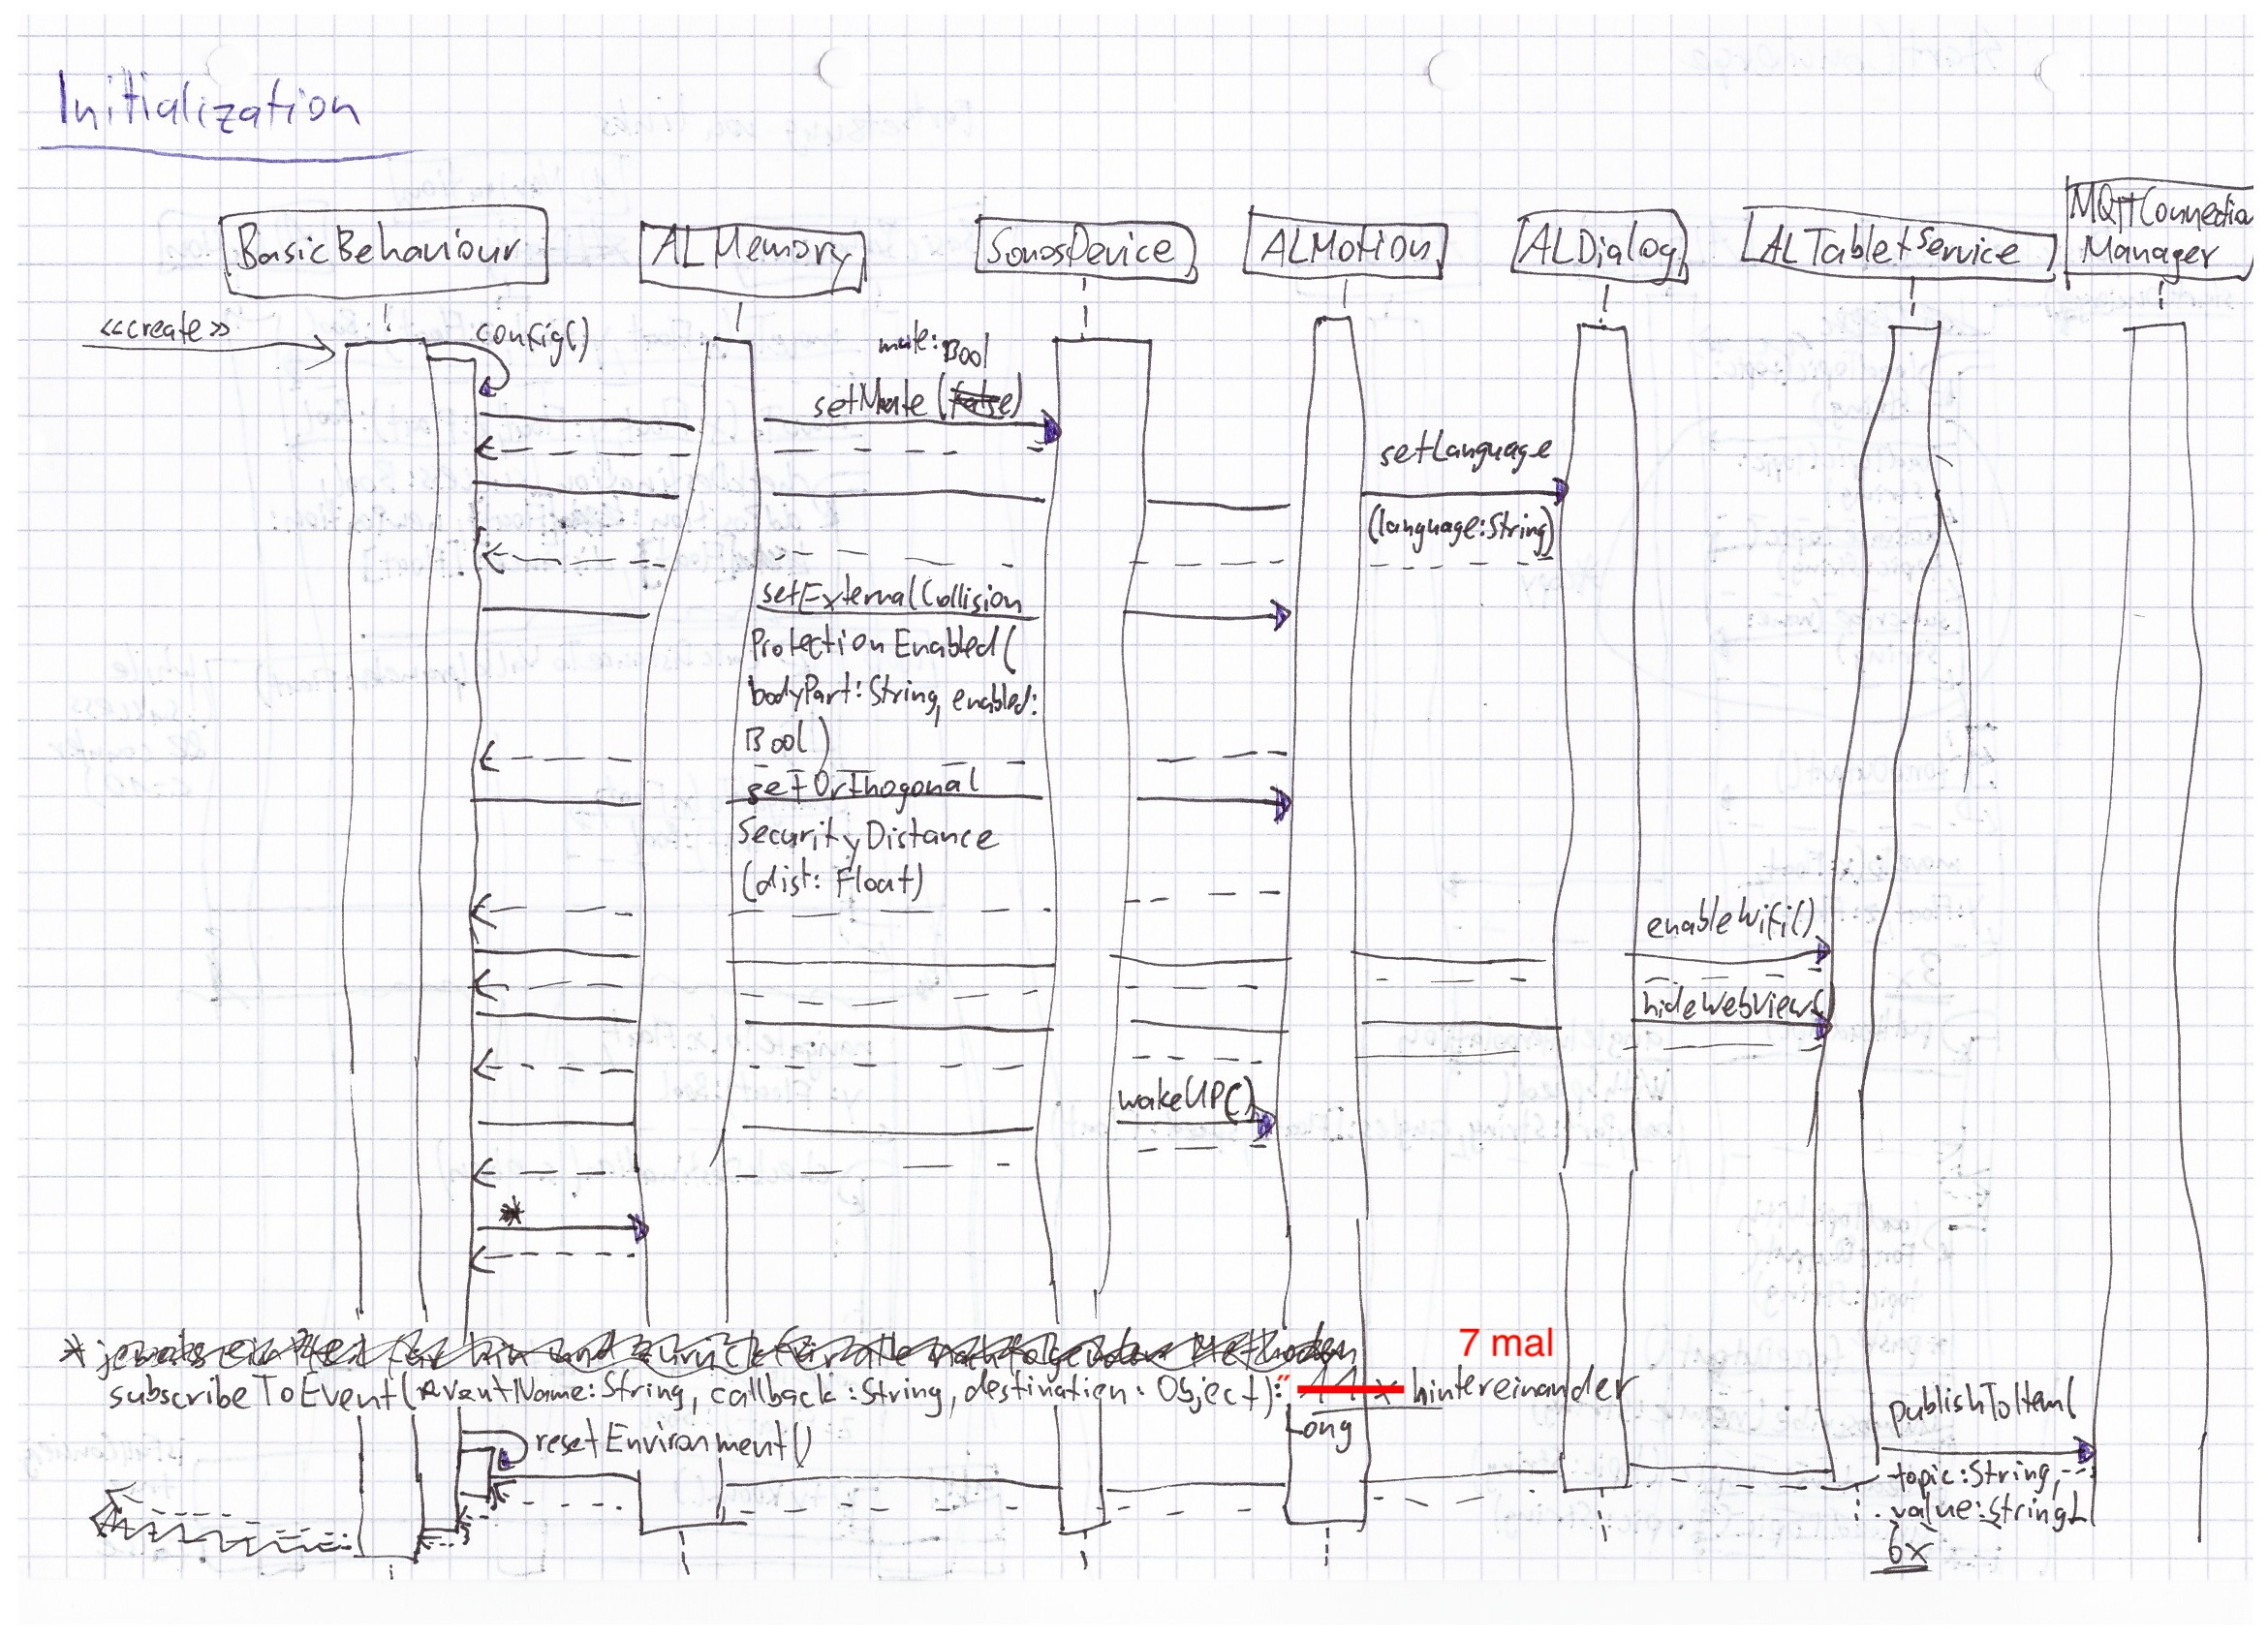
\includegraphics[width=\textwidth]{Scan_1.jpeg}
	\caption{Sequenzdiagramm - Initialisierung mit Standardwerten}
	\label{fig:sqd:classInitialization}
\end{figure}

\section{Führung}
\subsection{Start der Führung}
\label{subsec:startConcierge}
Die Führung beginnt mit einer Sprachausgabe. Hierfür wird die Klasse \lstinline|ALDialog| benötigt. Beim Start und beim Beenden der Sprachausgabe ist sehr genau auf die Reihenfolge der Aufrufe zu achten, sonst kann möglicherweise die Sprachsteuerung nur durch einen Neustart des Roboters beendet und somit erneut verwendet werden! Zum Start der Sprachsteuerung mit einer Dialogdatei, muss die entsprechende Datei im angegebenen Verzeichnis auf dem Roboter liegen. Ein Remote-Verzeichnis wird nicht akzeptiert! Die Methode \lstinline|loadTopic(topic:String)| läd die entsprechende Dialogdatei (\lstinline|Welcome.top|). Die Methode \lstinline|activateTopic(topic: String)| aktiviert das angegebene Topic, sodass Sprachein- und -ausgaben durch dieses Topic abgearbeitet werden. Durch Aufruf von \lstinline|subscribe(name:String)| wird die Sprachein- und -ausgabe auf dem Roboter aktiviert, sodass nun mit dem Roboter gesprochen werden kann. \lstinline|forceOutput| ermöglicht die Ausgabe der nächsten Phrase, welche durch \lstinline|proposal| in der Dialogdatei gekennzeichnet ist. Zum Beenden der Sprachsteuerung mit einer Dialogdatei muss zunächst durch \lstinline|unsubscribe(name:String)| die Sprachsteuerung auf dem Roboter deaktiviert werden. Die Methode \lstinline|deactivateTopic(topic:String)| deaktiviert das zuvor aktivierte Topic und mithilfe von \lstinline|unloadTopic(topic:String)| wird die geladene Dialogdatei freigegeben, sodass mit Durchführung der oben genannten Befehle wieder eine neue Dialogdatei eingelesen werden kann.\\
Die Methode \lstinline|moveTo(x:Float, y:Float, theta: Float): Bool| der Klasse \lstinline|ALMotion| ermöglicht die Fortbewegung des Roboters in die x- und y-Richtung. Durch Angabe des Theta-Wertes wird eine Drehung des Roboters ermöglicht. Hier erfolgt zunächst eine 180\textdegree-Drehung, eine Fortbewegung in x-Richtung, sowie eine erneute 180\textdegree-Drehung. Durch Aufruf der Methode \lstinline|putHeadUp()| unter der Verwendung der Methode \lstinline|angleInterpolationWithSpeed(bodyPart: String, angles: [Float], speed: Float)| wird der Kopf des Roboters in eine senkrechte Position gesetzt, sodass er auf die Personen, welche an der Führung teilnehmen, gerichtet ist. Die Methode \lstinline|loadTopicWithForceOutput(topic:String)| kapselt die oben genannten Schritte zum laden und entladen einer Dialogdatei inklusive der Ausgabe des ersten \lstinline|proposals| der jeweiligen Datei. Hier wird die Datei \lstinline|General.top| geladen.\\
Im Anschluss wird die Tour in Richtung des TV Raumes fortgesetzt durch eine 90\textdegree-Drehung im Uhrzeigersinn, sowie einer Bewegung in x-Richtung. Bei wichtigen Strecken folgt ein Aufruf der Methode \lstinline|checkDestination(success: Bool, oldPosition: [Float], newPosition: [Float], distance: [Float])|, welche bei nicht Ankunft am Ziel, aufgrund zum Beispiel von Hindernissen, die Strecke, die noch zurückzulegen ist bist zum Ziel, berechnet und diese unter der Verwendung der Methode \lstinline|navigateTo(x: Float, y: Float): Bool| versucht zurückzulegen. Die Methode \lstinline|navigateTo| ermöglicht bestmöglichst die Umfahrung von Hindernissen auf dem Weg. Da bei nicht Ankunft am Ziel ein Fehlerstatus im Hintergrund vorhanden ist, welche über die weitere Fortbewegung des Roboters entscheidet und es eine unbestimmte Zeit benötigt, bis dieser wieder zurückgesetzt ist, wird die Interpolation der Fortbewegung des Roboters bis zu zehn Mal versucht oder bis er am Ziel angekommen ist. \\
Am Ende eines jeden Raumes wird bestimmt, ob der nachfolgende Raum ebenfalls ausgeführt werden soll oder nicht. Dies kann durch das Menü (siehe Abschnitt \ref{sec:startApp}) gesteuert werden. 

\begin{figure}[ht]
	\centering
	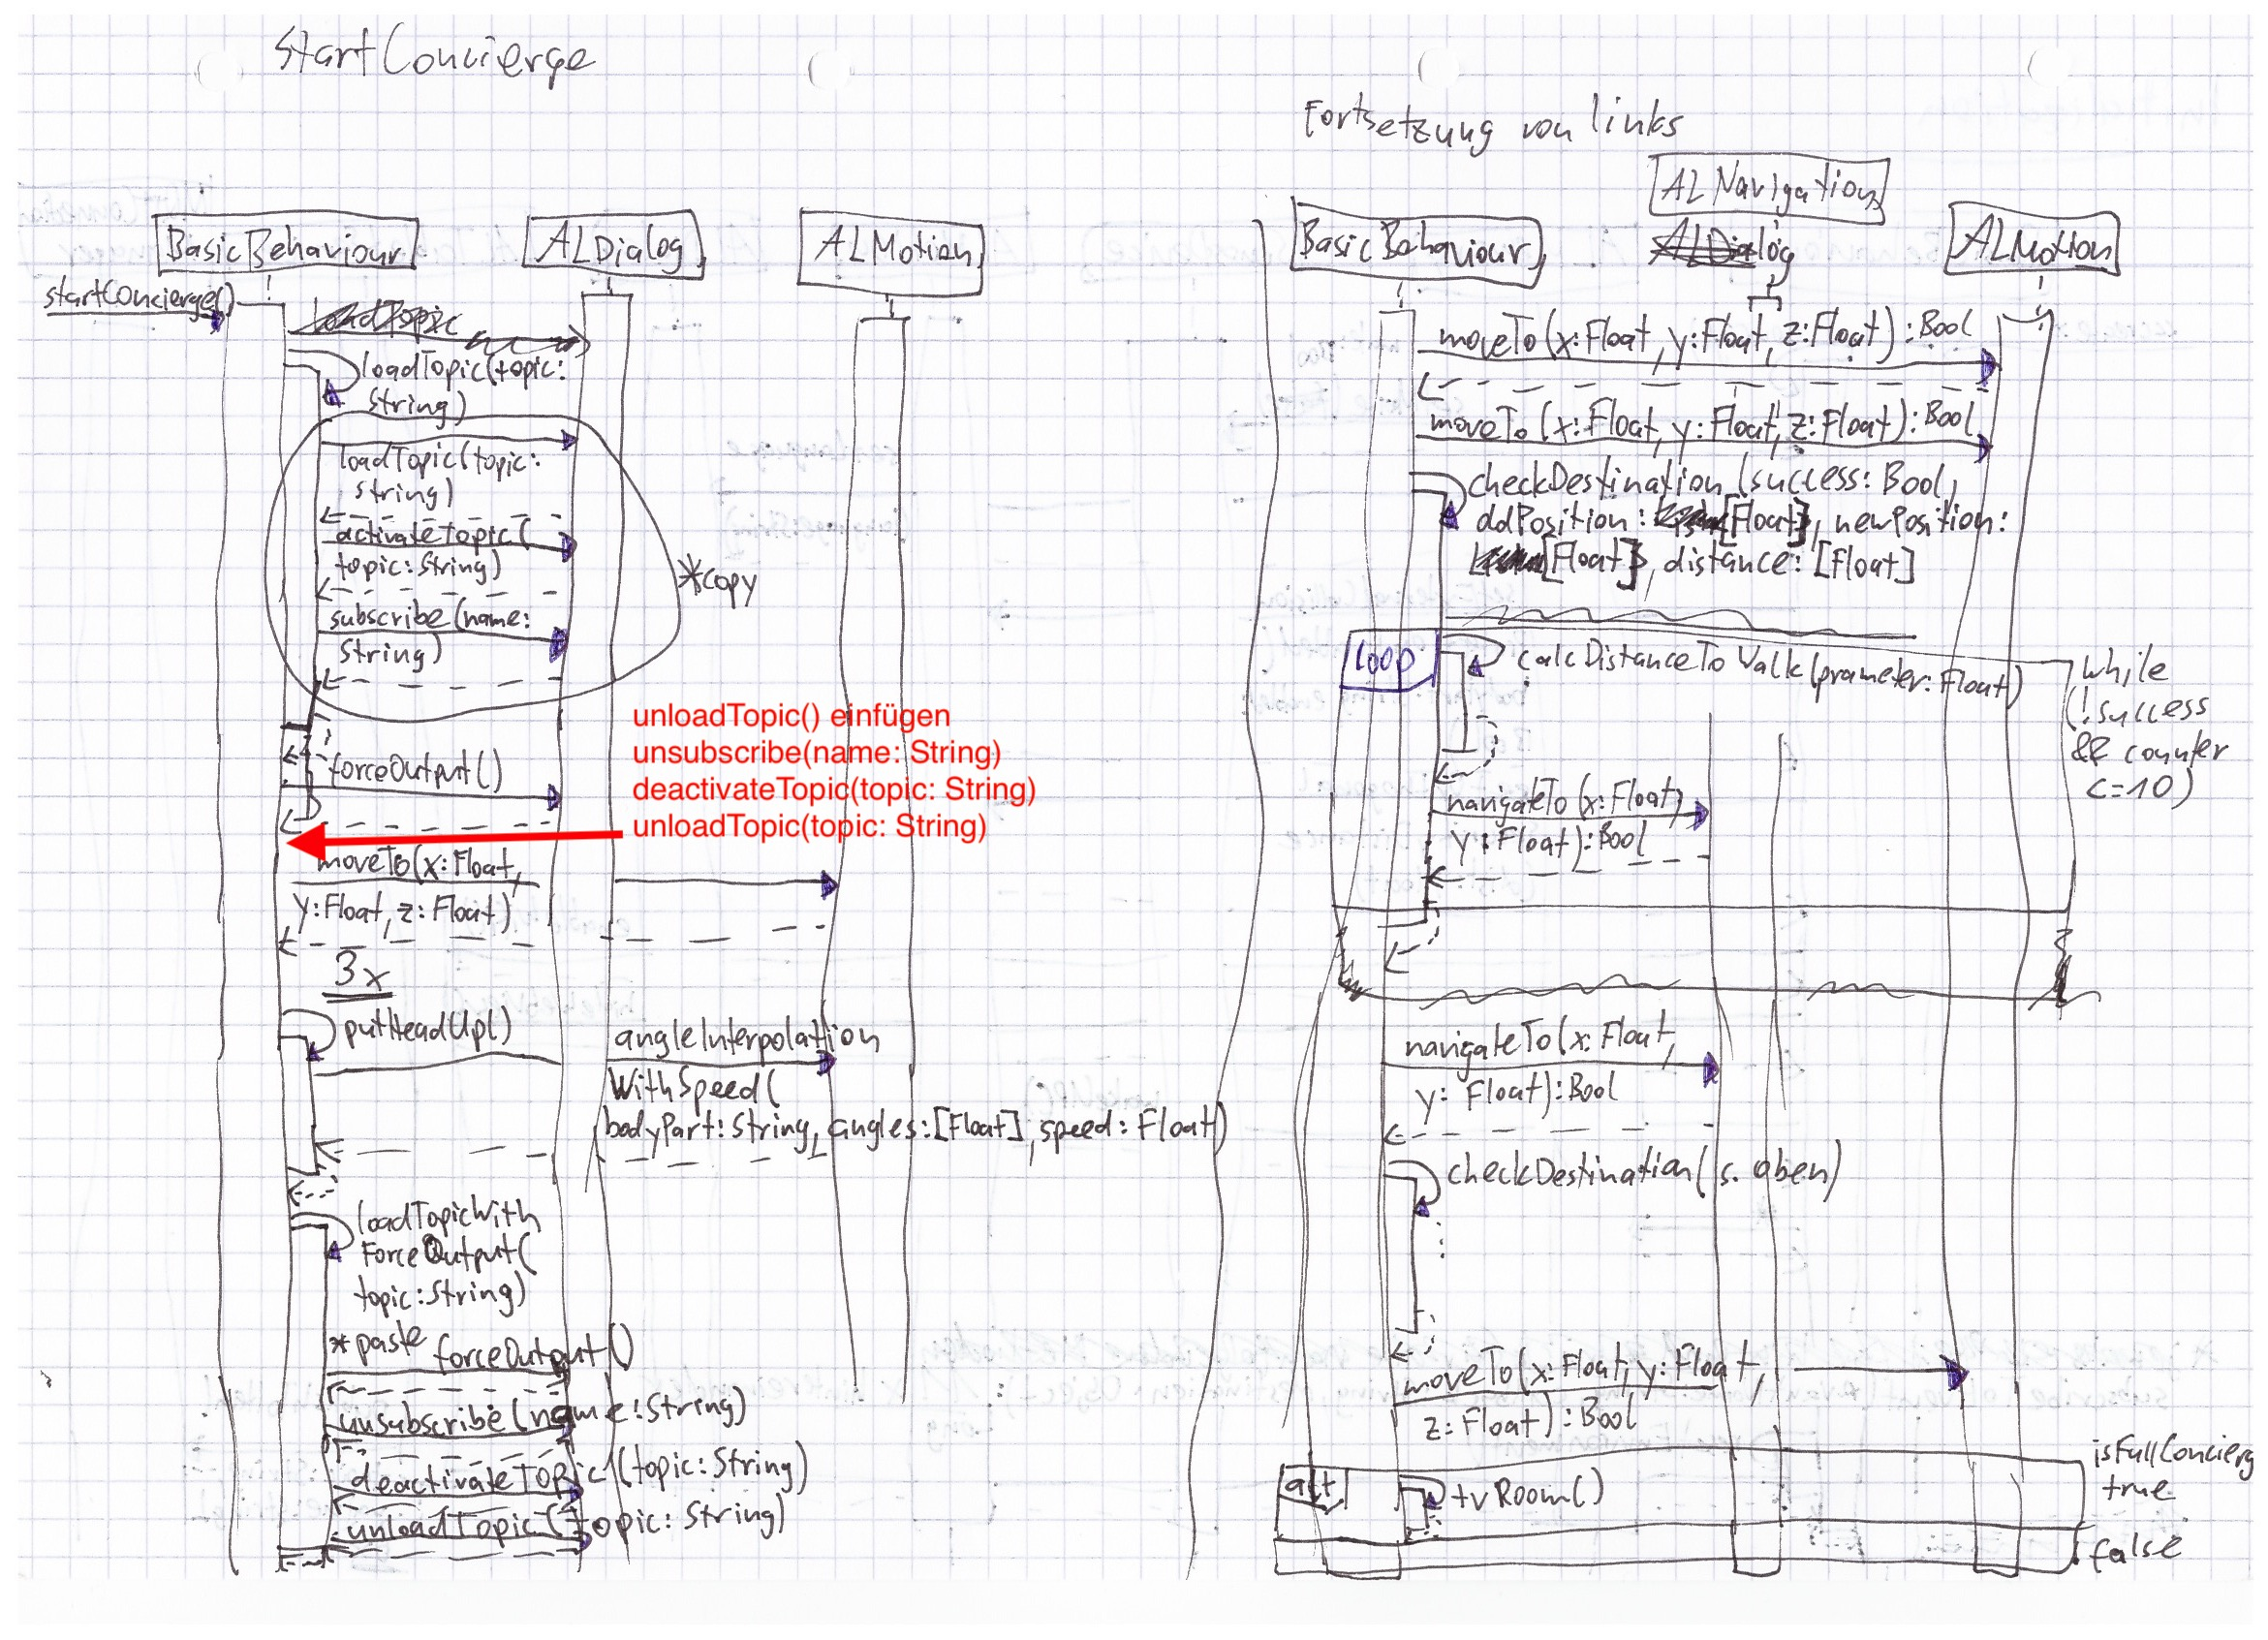
\includegraphics[width=\textwidth]{Scan_2.jpeg}
	\caption{Sequenzdiagramm - Start der Führung}
	\label{fig:sqd:startConcierge}
\end{figure}

\subsection{TV Raum}
\label{subsec:tvRoom}
Im TV Raum werden zu Beginn zwei Events bei der Klasse \lstinline|ALMemory| registriert, welche ausgelöst werden, wenn ein Fenster geöffnet bzw. geschlossen wird. Ebenso werden die MQTT-Topics aller Fenster abonniert, sodass eine Reaktion auf das Öffnen oder Schließen eines der Fensters ausgeführt werden kann. Nach dem Laden der Dialogdatei (\lstinline|TVRoom.top|) und der Sprachausgabe des Roboters wird auf das Öffnen eine Fensters gewartet. Sobald ein Fenster geöffnet wird, wird die Callback-Methode \lstinline|onSubscription(item: String, value: String)| aufgerufen. Hier wird entschieden, ob ein Fenster geöffnet oder geschlossen wurde. Bei Öffnen eines Fensters wird das entsprechende Event der Klasse \lstinline|ALMemory| ausgelöst, welches eine weitere Sprachausgabe des Roboters ausführt und das Abonnement dieses Events beendet. Nach Schließen eines Fensters wird ebenso das jeweilige Event ausgelöst, welches wiederum eine Sprachausgabe und das Beenden des Abonnements des Events zur Folge hat. 

\begin{figure}[ht]
	\centering
	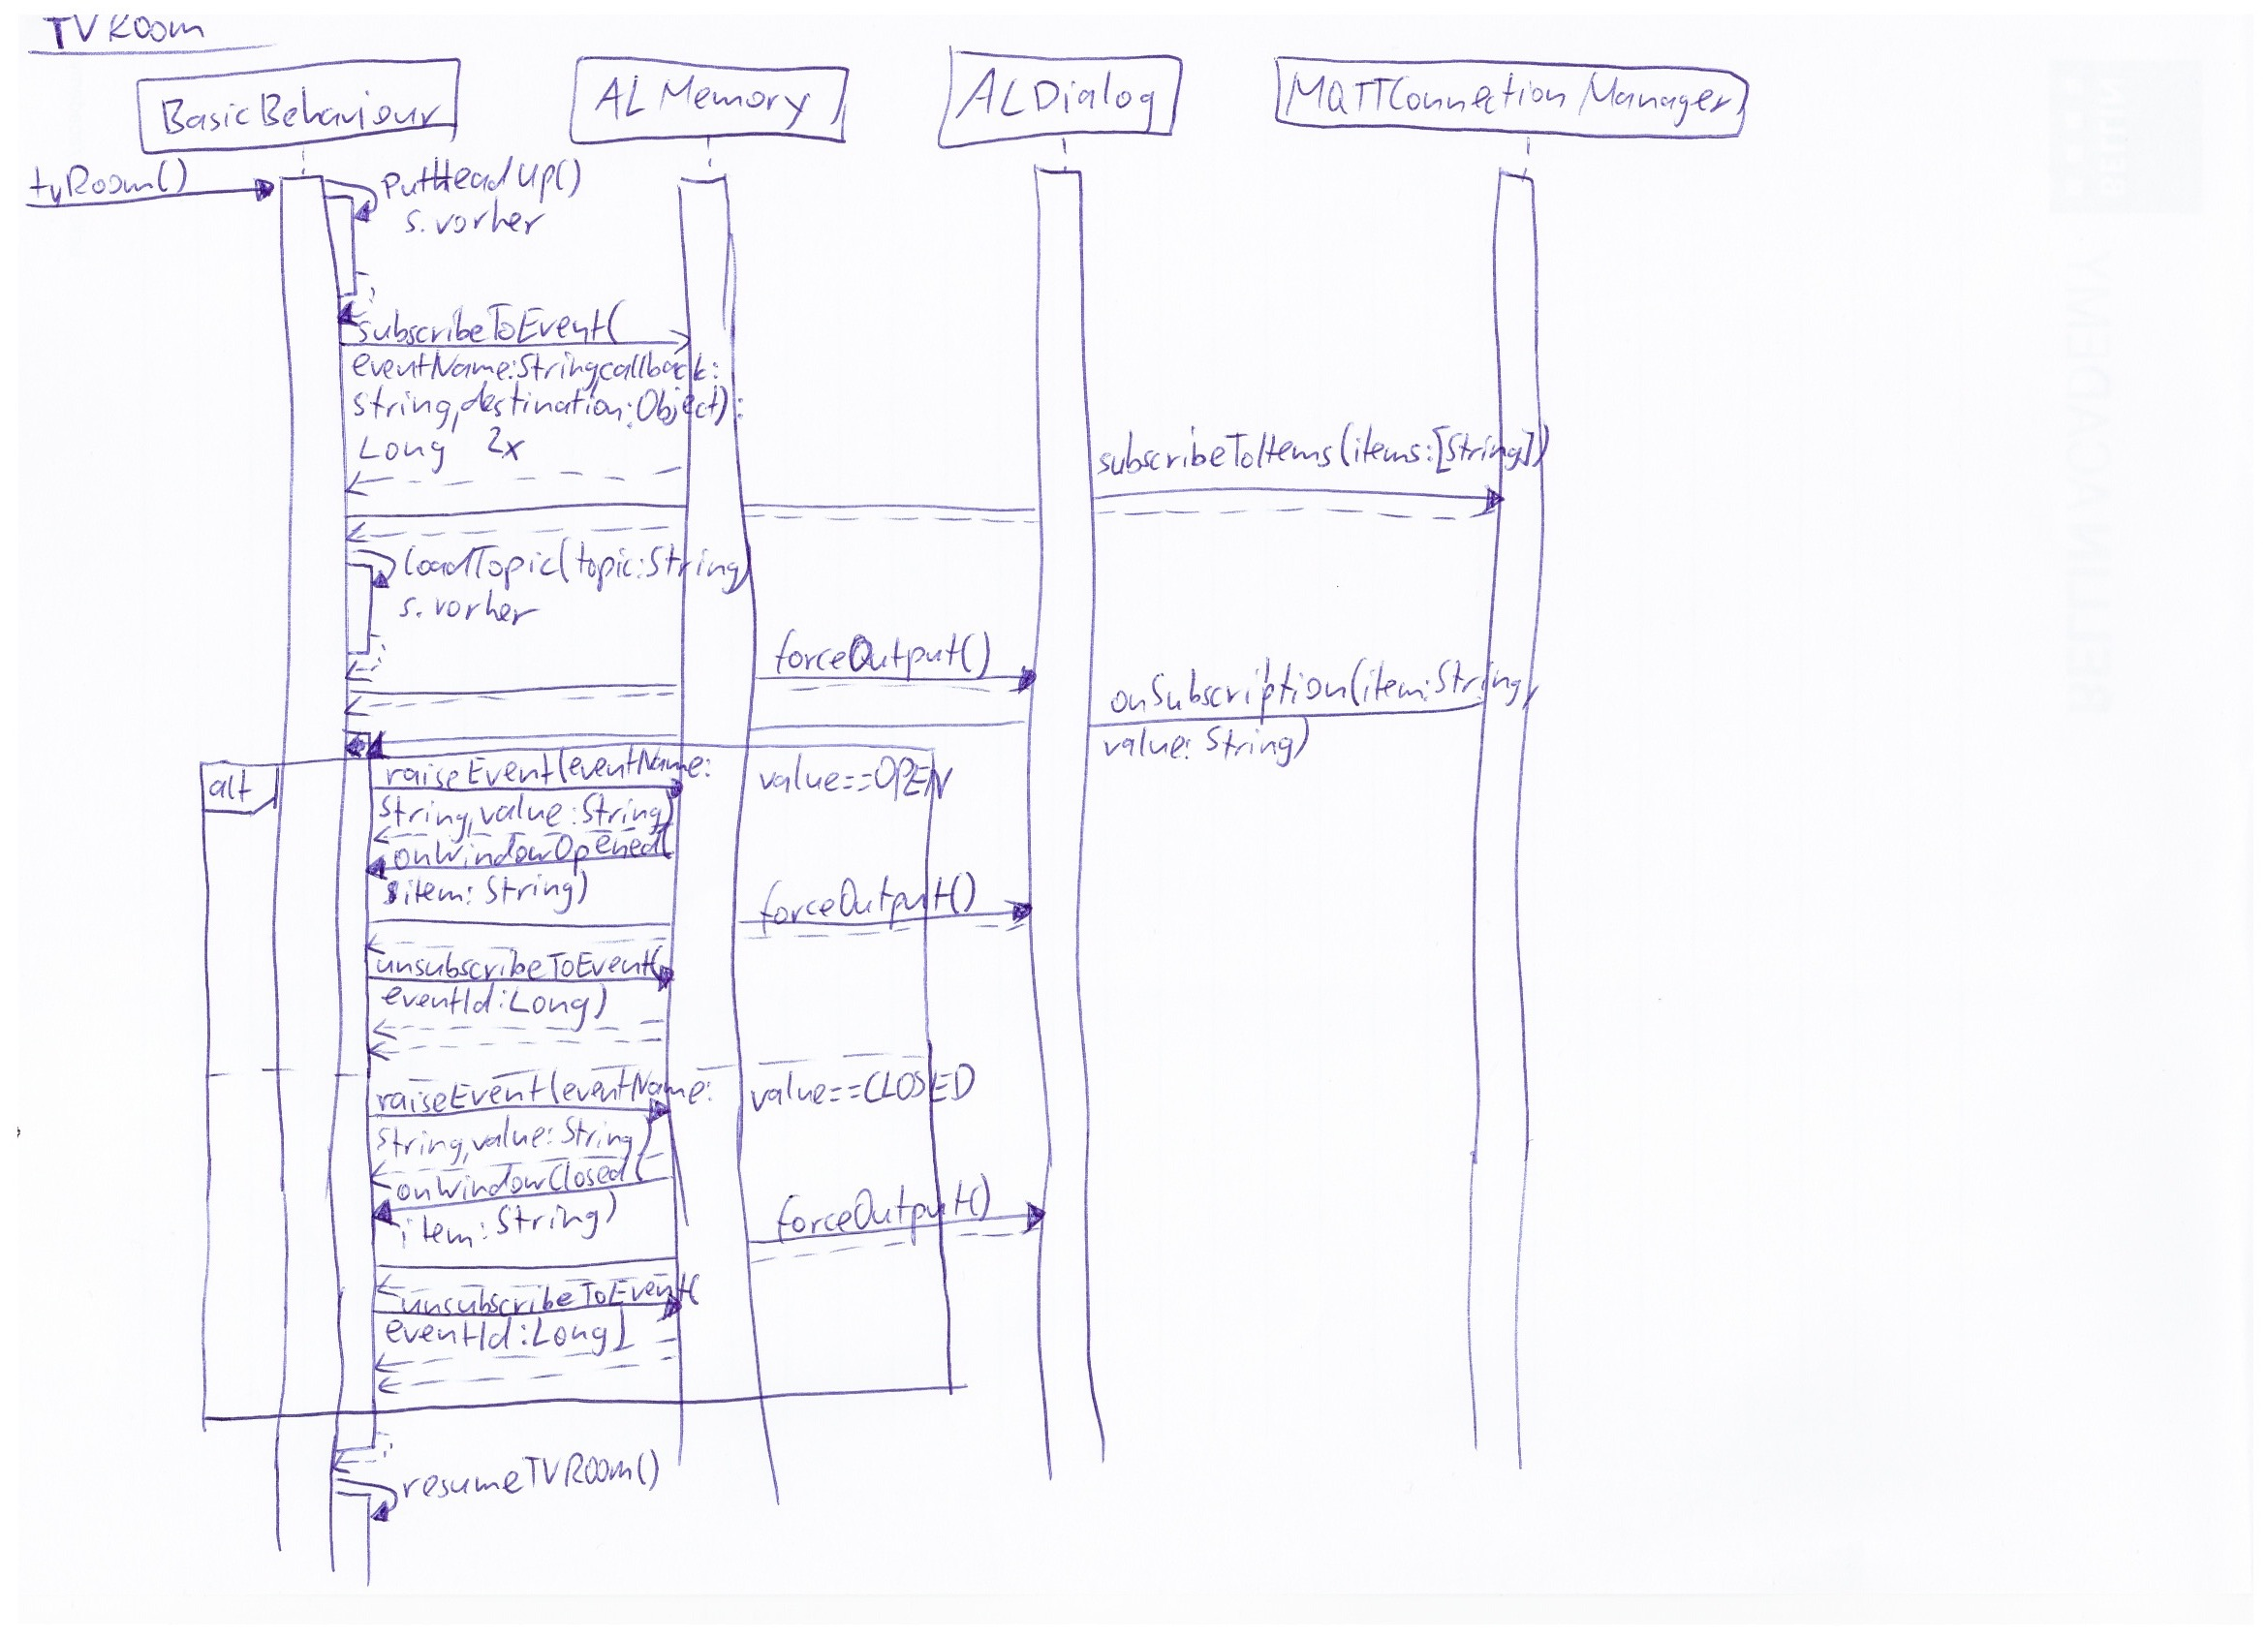
\includegraphics[width=\textwidth]{Scan_3.jpeg}
	\caption{Sequenzdiagramm - Führung im TV Raum Teil 1}
	\label{fig:sqd:tvRoom}
\end{figure}

Im Anschluss wird die Führung des TV Raumes durch Aufruf der Methode \lstinline|resumeTVRoom()| fortgeführt. Die Abonnements der MQTT-Topics aller Fenster werden ebenso beendet. Danach folgt die Spieleszene (\lstinline|runGamingScene()|). Durch den asynchronen Aufruf der Methode \lstinline|getRequest(url:String)| der Klasse \lstinline|ConnectionManager| erfolgt das Abspielen eines Videos auf dem Fernseher. Hierbei wird die entsprechende Url, welche in der Konfigurationsdatei hinterlegt ist (siehe Abschnitt \ref{subsec:configFile}) verwendet. Parallel dazu wird noch mithilfe der Klasse \lstinline|ALAnimationPlayer| eine Animation des Roboters abgespielt (\lstinline|run(animation:String)|). Danach folgen weitere Sprachausgaben des Roboters, sowie das Beenden des Dialoges. Durch eine Reihe weiterer \lstinline|navigateTo(x: Float, y: Float): Bool| Befehle erfolgt der Positionswechsel in das Arbeitszimmer. Die navigateTo-Befehle beinhalten zuerst eine Bewegung in x-Richtung, eine 90\textdegree-Drehung im Uhrzeigersinn, eine weitere Bewegung in x-Richtung, sowie eine weitere 90\textdegree-Drehung im Uhrzeigersinn und eine erneute Bewegung in x-Richtung. Bei Ankunft erfolgt noch eine 180\textdegree-Drehung, um sich dem Publikum wieder zuzuwenden. Dort angekommen wird abgeprüft, ob die Tour weiter fortgesetzt, oder beendet werden soll (siehe Abschnitt \ref{sec:startApp}).

\begin{figure}[ht]
	\centering
	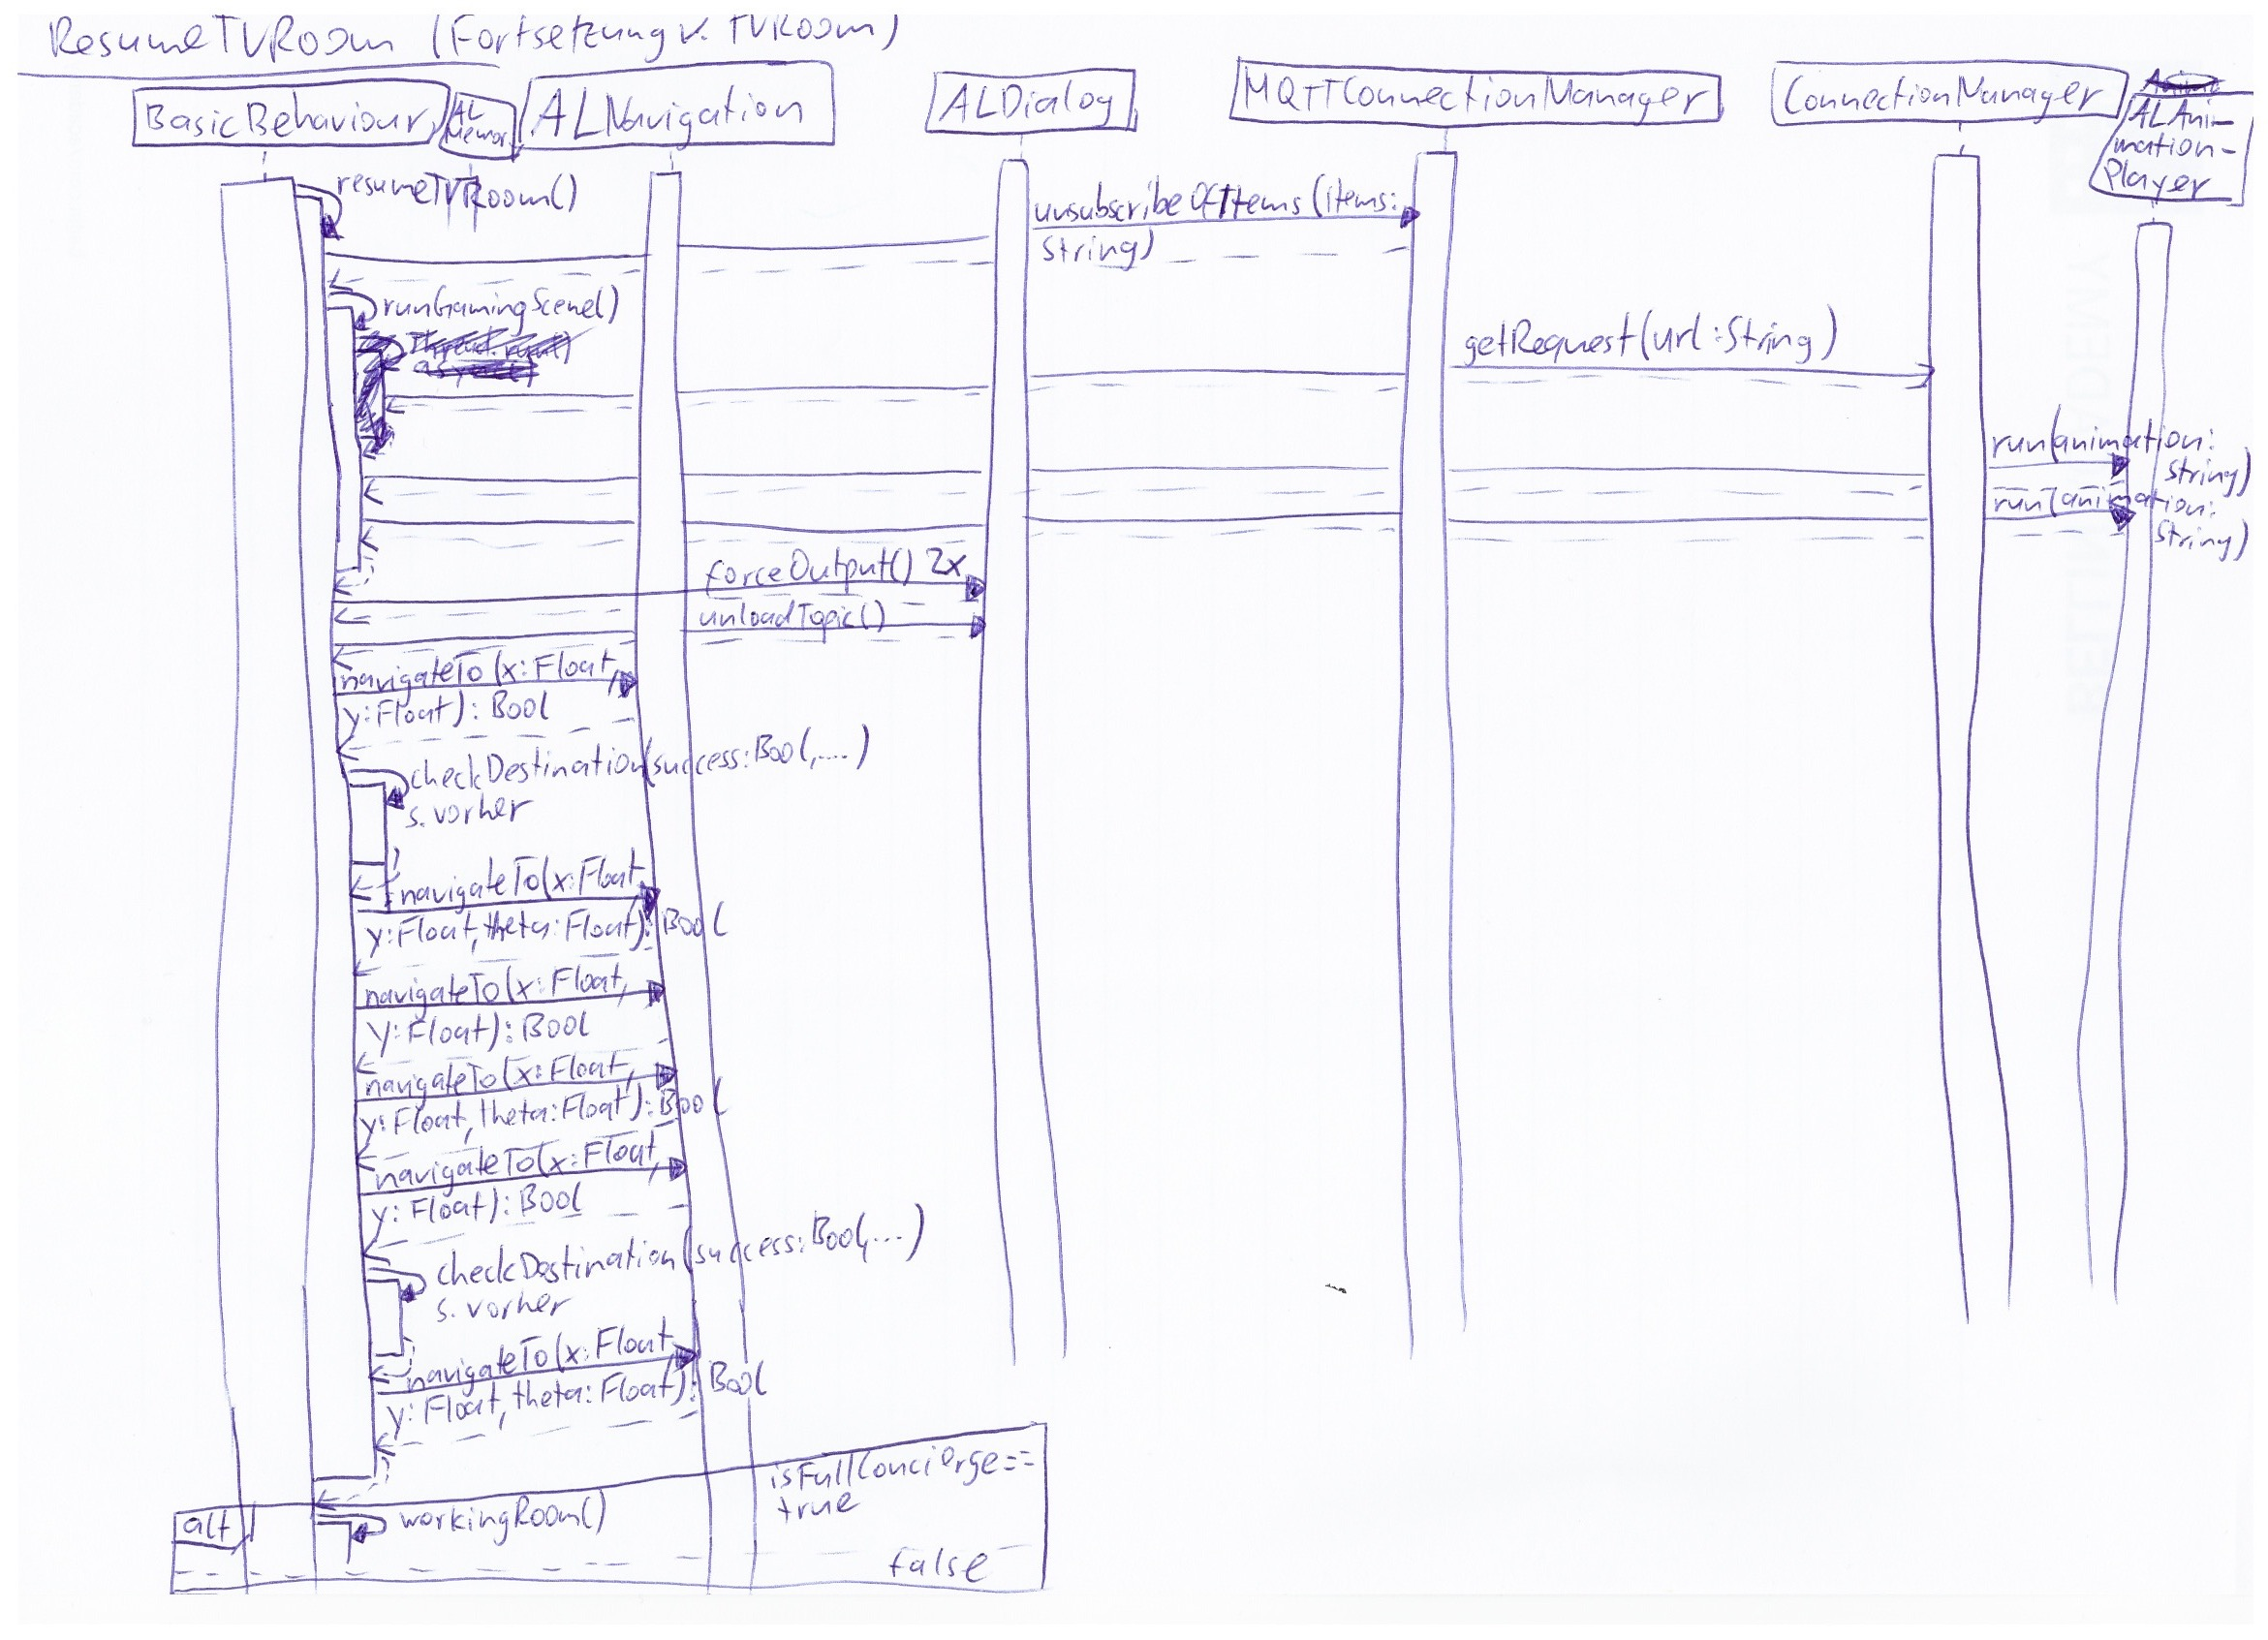
\includegraphics[width=\textwidth]{Scan_4.jpeg}
	\caption{Sequenzdiagramm - Führung im TV Raum Teil 2}
	\label{fig:sqd:resumeTvRoom}
\end{figure}

\subsection{Arbeitszimmer}
Im Arbeitszimmer wird wie auch bei alle den anderen Räumen und Positionen zuerst Peppers Kopf in eine senkrechte Position versetzt, durch Aufrufen der Methode \lstinline|putHeadUp()|. Im Anschluss wird die entsprechende Dialogdatei \lstinline|WorkingRoom.top| geladen, das darin enthaltene \lstinline|proposal| wiedergegeben und das Topic wieder entladen. Danach erfolgt der Positionswechsel in das Badezimmer. Hierfür wird zunächst eine Bewegung in x-Richtung mithilfe eines Aufrufes von \lstinline|moveTo(x: Float, y: Float, theta: Float): Bool| getätigt, gefolgt von einer Überprüfung über die Ankunft am Ziel, sowie eine mögliche Interpolation an das geplante Ziel (\lstinline|checkDestination(success: Bool, oldPosition: [Float], newPosition: [Float], distance: [Float])|). Nach einer 90\textdegree-Drehung im Uhrzeigersinn wird die Bewegung in x-Richtung fortgesetzt, um das Badezimmer zu betreten, ebenfalls gefolgt von einer Überprüfung über die Ankunft am Ziel. Ist der Roboter im Badezimmer angekommen, so tätigt er eine 180\textdegree-Drehung und wendet sich den Teilnehmern der Führung wieder zu. Wie auch bei den vorherigen Räumen wird überprüft, ob der aktuelle Raum, in diesem Fall das Badezimmer ebenso durchgeführt werden soll oder nicht (siehe Abschnitt \ref{sec:startApp}).

\begin{figure}[ht]
	\centering
	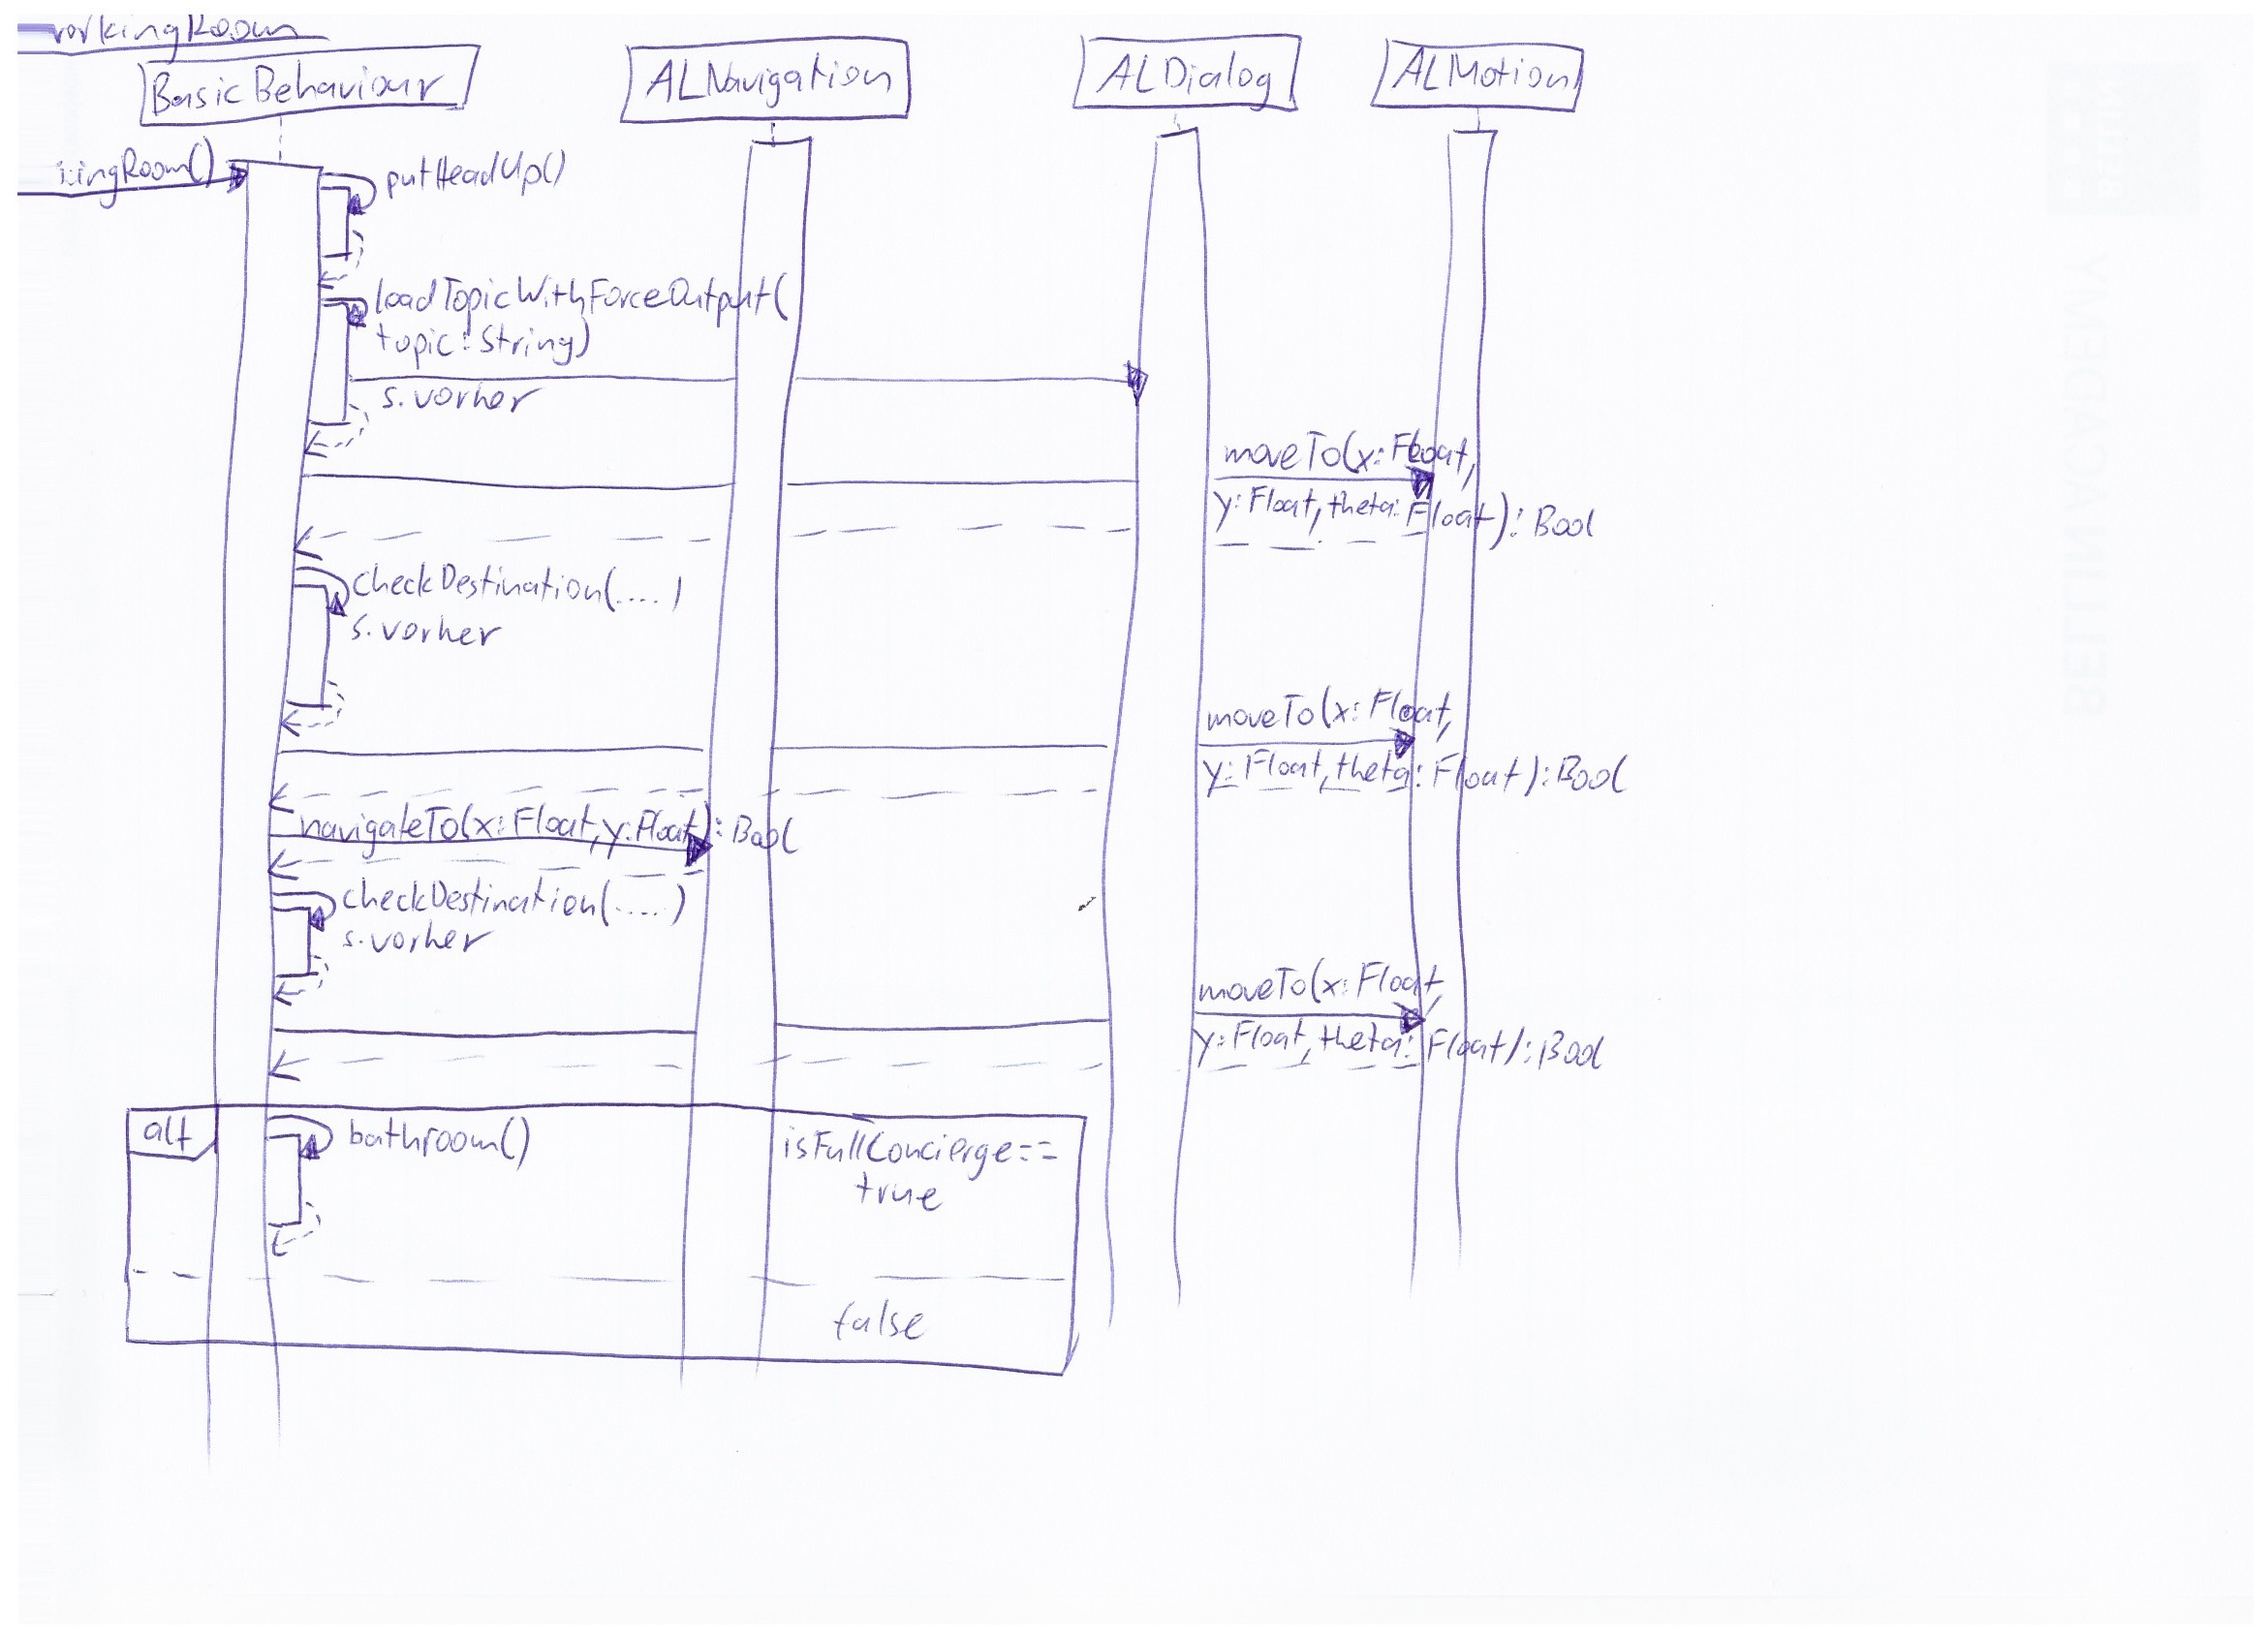
\includegraphics[width=\textwidth]{Scan_5.jpeg}
	\caption{Sequenzdiagramm - Führung im Arbeitszimmer}
	\label{fig:sqd:workingroom}
\end{figure}

\subsection{Badezimmer}
\label{subsec:bathroom}
Zu Beginn im Badezimmer wird der Kopf des Roboters in eine senkrechte Position versetzt. Danach wird die entsprechende Dialogdatei \lstinline|Bathroom.top| geladen und die erste Sprachausgabe getätigt. Innerhalb des ersten \lstinline|proposals| wird das Event \lstinline|GetValue| (siehe Abschnitt \ref{sec:initialization}) ausgelöst und somit der Temperaturwert von OpenHab (\lstinline|openHabGetRequest(mqttTopic: String, key:String): [String]|) abgerufen und in \lstinline|ALMemory| gespeichert. Innerhalb des gleichen \lstinline|proposals| wird der abgerufene Wert aus dem Speicher geladen und vom Roboter dynamisch wiedergegeben. Im Anschluss folgen weitere zwei Sprachausgaben (\lstinline|forceOutput()|), wobei die letzte eine Interaktion mit dem Sprachassistenten \glqq Alexa\grqq\xspace darstellt. Nach dem entladen der Dialogdatei folgt die Navigation in die Küche. Hierfür werden, wie in Abbildung \ref{fig:sqd:bathroom} zu sehen ist, einige Funktionsaufrufe von \lstinline|moveTo(x: Float, y: Float, theta: Float): Bool|, \lstinline|navigateTo(x: Float, y: Float)| und \lstinline|checkDestination(success: Bool, oldPosition: [Float], newPosition: [Float], distance: [Float])| durchgeführt. Zuerst erfolgt eine Bewegung in x-Richtung, gefolgt von einer 90\textdegree-Drehung im Uhrzeigersinn, sowie einer Navigation in x-Richtung, ebenfalls gefolgt von einer weiteren 90\textdegree-Drehung im Uhrzeigersinn, einer weiteren Navigation in x-Richtung und bei Ankunft am Ziel eine 180\textdegree-Drehung, damit Pepper wieder in Richtung des Publikums schaut. Eine Überprüfung über die weitere Durchführung der Führung beendet den Abschnitt des Badezimmers.


\begin{figure}[ht]
	\centering
	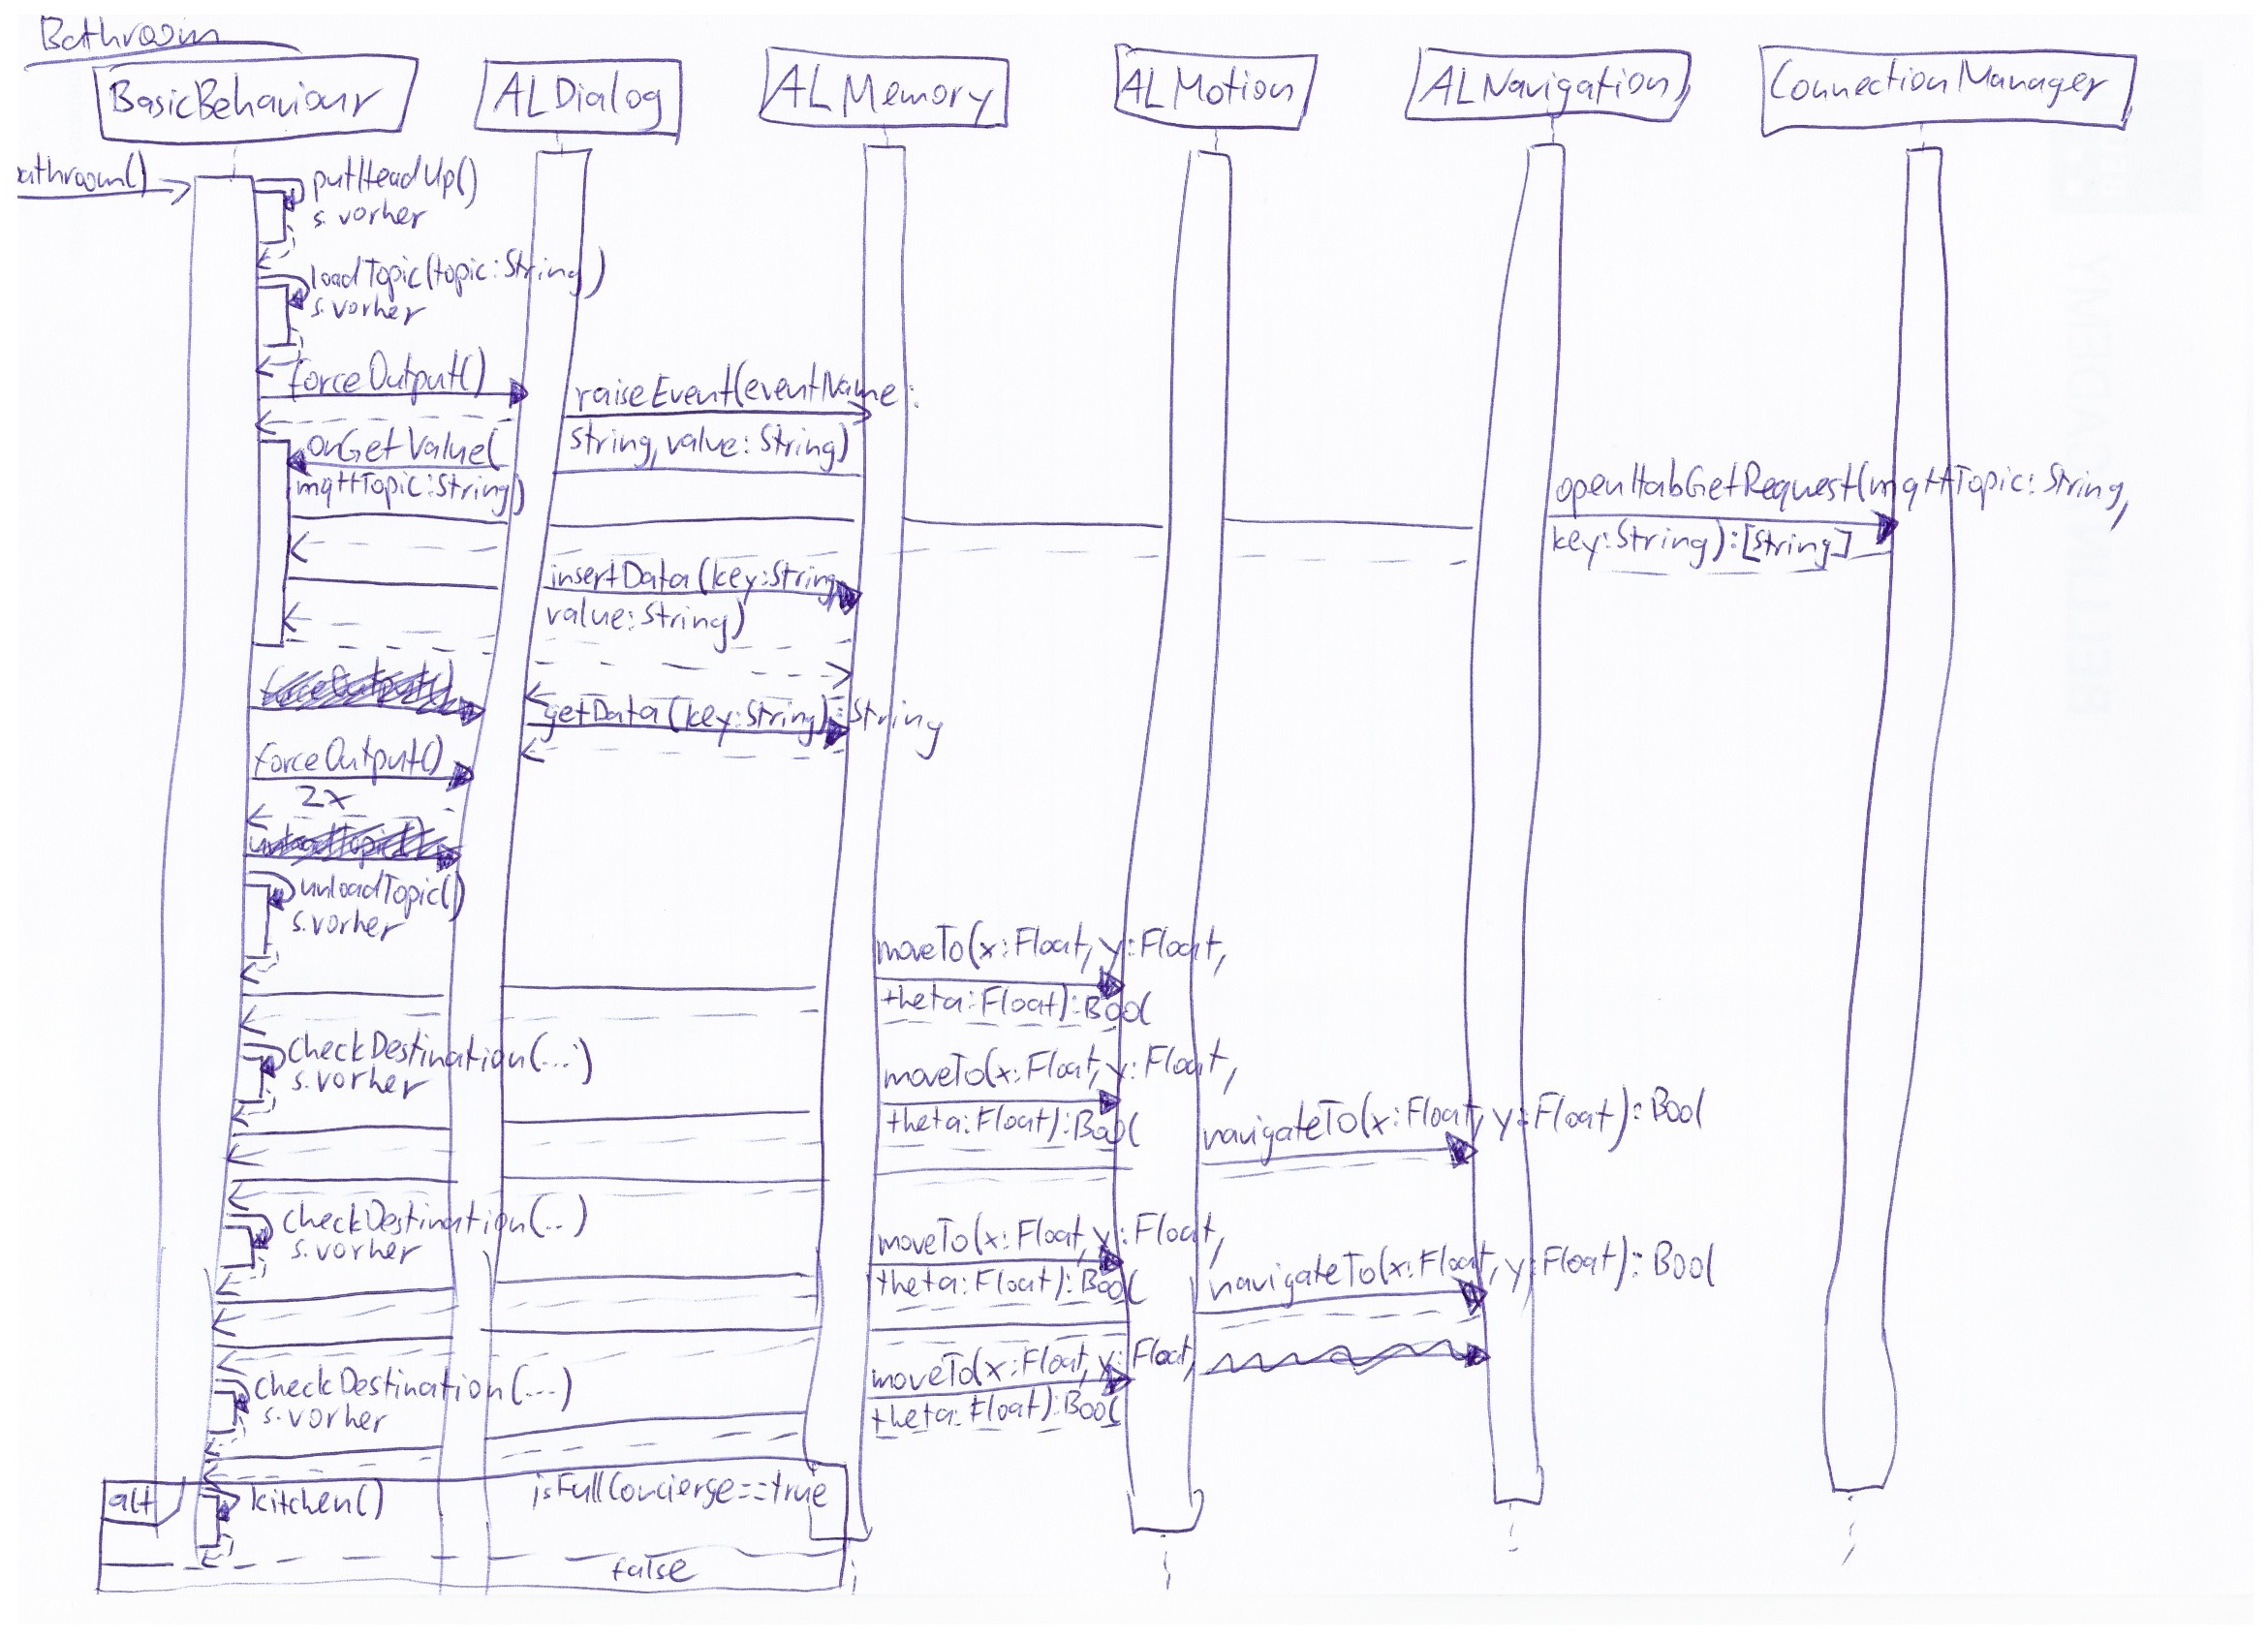
\includegraphics[width=\textwidth]{Scan_6.jpeg}
	\caption{Sequenzdiagramm - Führung im Badezimmer}
	\label{fig:sqd:bathroom}
\end{figure}

\subsection{Küche}
Der Beginn der Führung in der Küche ist weitgehend identisch mit dem des Badezimmers (siehe Abschnitt \ref{subsec:bathroom}). Von der Positionierung des Kopfes des Roboters, über das Laden der Dialogdatei (\lstinline|Kitchen.top|), sowie das Abrufen der Kühlschranktemperatur über OpenHab, Speichern in \lstinline|ALMemory|) und dynamisches Abrufen des Wertes und einbauen in die Sprachausgabe ergibt sich kein relevanter Unterschied. Die Navigation aus der Küchen in den Empfangsbereich wird durch eine Reihe von \lstinline|moveTo(x: Float, y: Float, theta: Float): Bool|-Befehlen (siehe Abbildung \ref{fig:sqd:kitchen} realisiert. Die Navigation baut sich wie folgt auf: eine Bewegung in x-Richtung, gefolgt von einer 90\textdegree-Drehung im Uhrzeigersinn, einer weiteren Bewegung in x-Richtung und einer abschließenden 180\textdegree-Drehung. Zum Schluss wird wie nach jedem Raum die Fortführung der Tour überprüft und gegebenenfalls fortgesetzt.

\begin{figure}[ht]
	\centering
	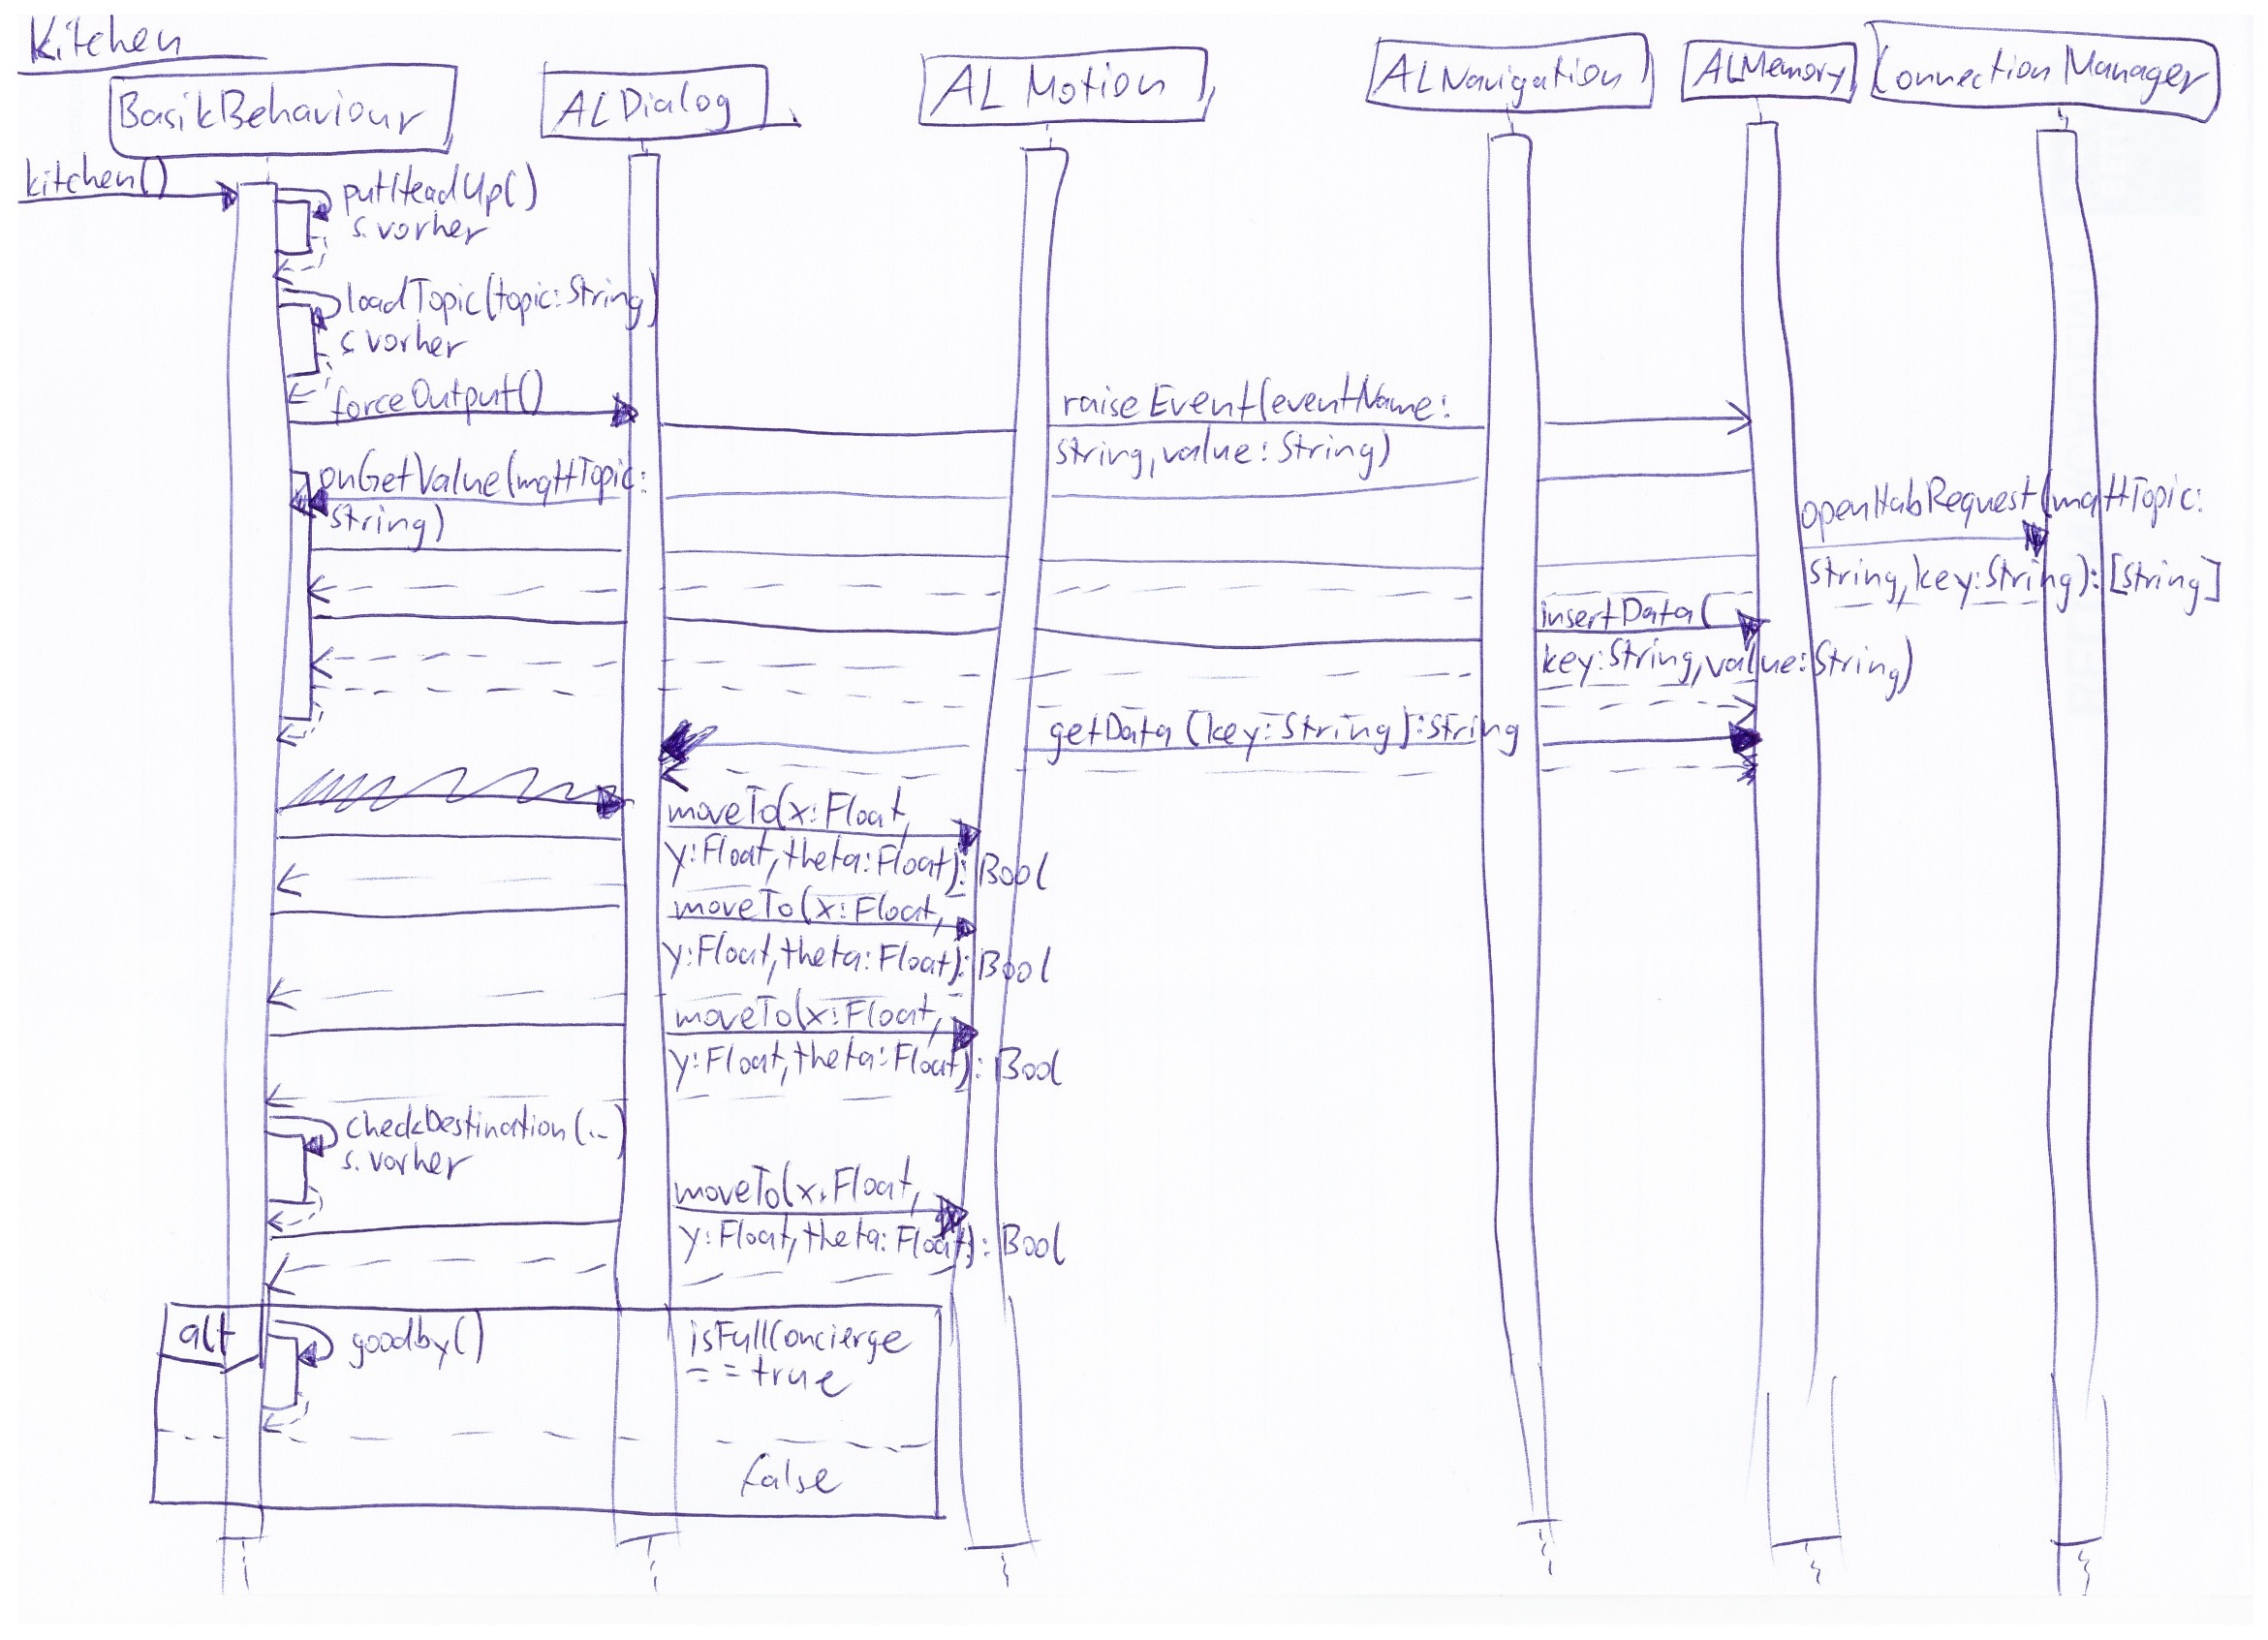
\includegraphics[width=\textwidth]{Scan_7.jpeg}
	\caption{Sequenzdiagramm - Führung in der Küche}
	\label{fig:sqd:kitchen}
\end{figure}

\subsection{Abschlussszene}
\label{subsec:goodby}
Nach der Positionierung des Kopfes des Roboters, dem Laden der Dialogdatei \lstinline|Questions.top| und einer Sprachausgabe des Roboters erfolgt die sprachlicher Interaktion in Verbindung mit Pepper. Hierbei können die Besucher Pepper einige Fragen stellen oder Befehle ausführen lassen. Hierzu zählen zum Beispiel Fragen, wie \glqq Wie heißt du?\grqq, \glqq Wie alt bist du?\grqq\xspace oder \glqq Wie viele Geräte gibt es hier im Smart Home Labor?\grqq und Befehle wie \glqq Schalte das Licht ein\grqq\xspace oder \glqq Mach ein Bild\grqq. Die vollständige Liste an möglichen Fragen und Befehlen kann der oben genannten Dialogdatei entnommen werden. Durch die Spracheingabe des Wortes \glqq Ende\grqq\xspace und damit einhergehendes Auslösen des Events \lstinline|SpeechRecognitionOff| (siehe Abschnitt \ref{sec:initialization}) wird die Sprachsteuerung beendet und der Roboter setzt seine Tour fort. Zunächst wird durch Aufruf der Methoden \lstinline|loadUrl(url:String): Bool| und \lstinline|showWebview(): Bool| der Klasse \lstinline|ALTabletService| die Webseite für die Bewertung der Führung auf Peppers Tablet geladen und angezeigt. Die Url wird der Konfigurationsdatei (siehe Abschnitt \ref{subsec:configFile}) entnommen. Im Anschluss setzt der Roboter seine Sprachausgabe durch Laden der Dialogdatei \lstinline|Goodby.top| fort. Die Abschlussshow wird durch aufrufen der Methode \lstinline|lightShow()| durchgeführt. Der komplette Befehlsablauf der ist in Abbildung \ref{fig:sqd:goodby} aufgrund des Umfangs nicht aufgeführt. Hierbei handelt es sich um eine Menge an MQTT-Befehlen zur Steuerung der Rollläden, Lichter und Türen im Smart Home Labor mit musikalischer Untermalung. Nach der Abschlussshow folgt eine letzte Sprachausgabe des Roboters zur Beendigung der Tour und entladen der Dialogdatei. 

\begin{figure}[ht]
	\centering
	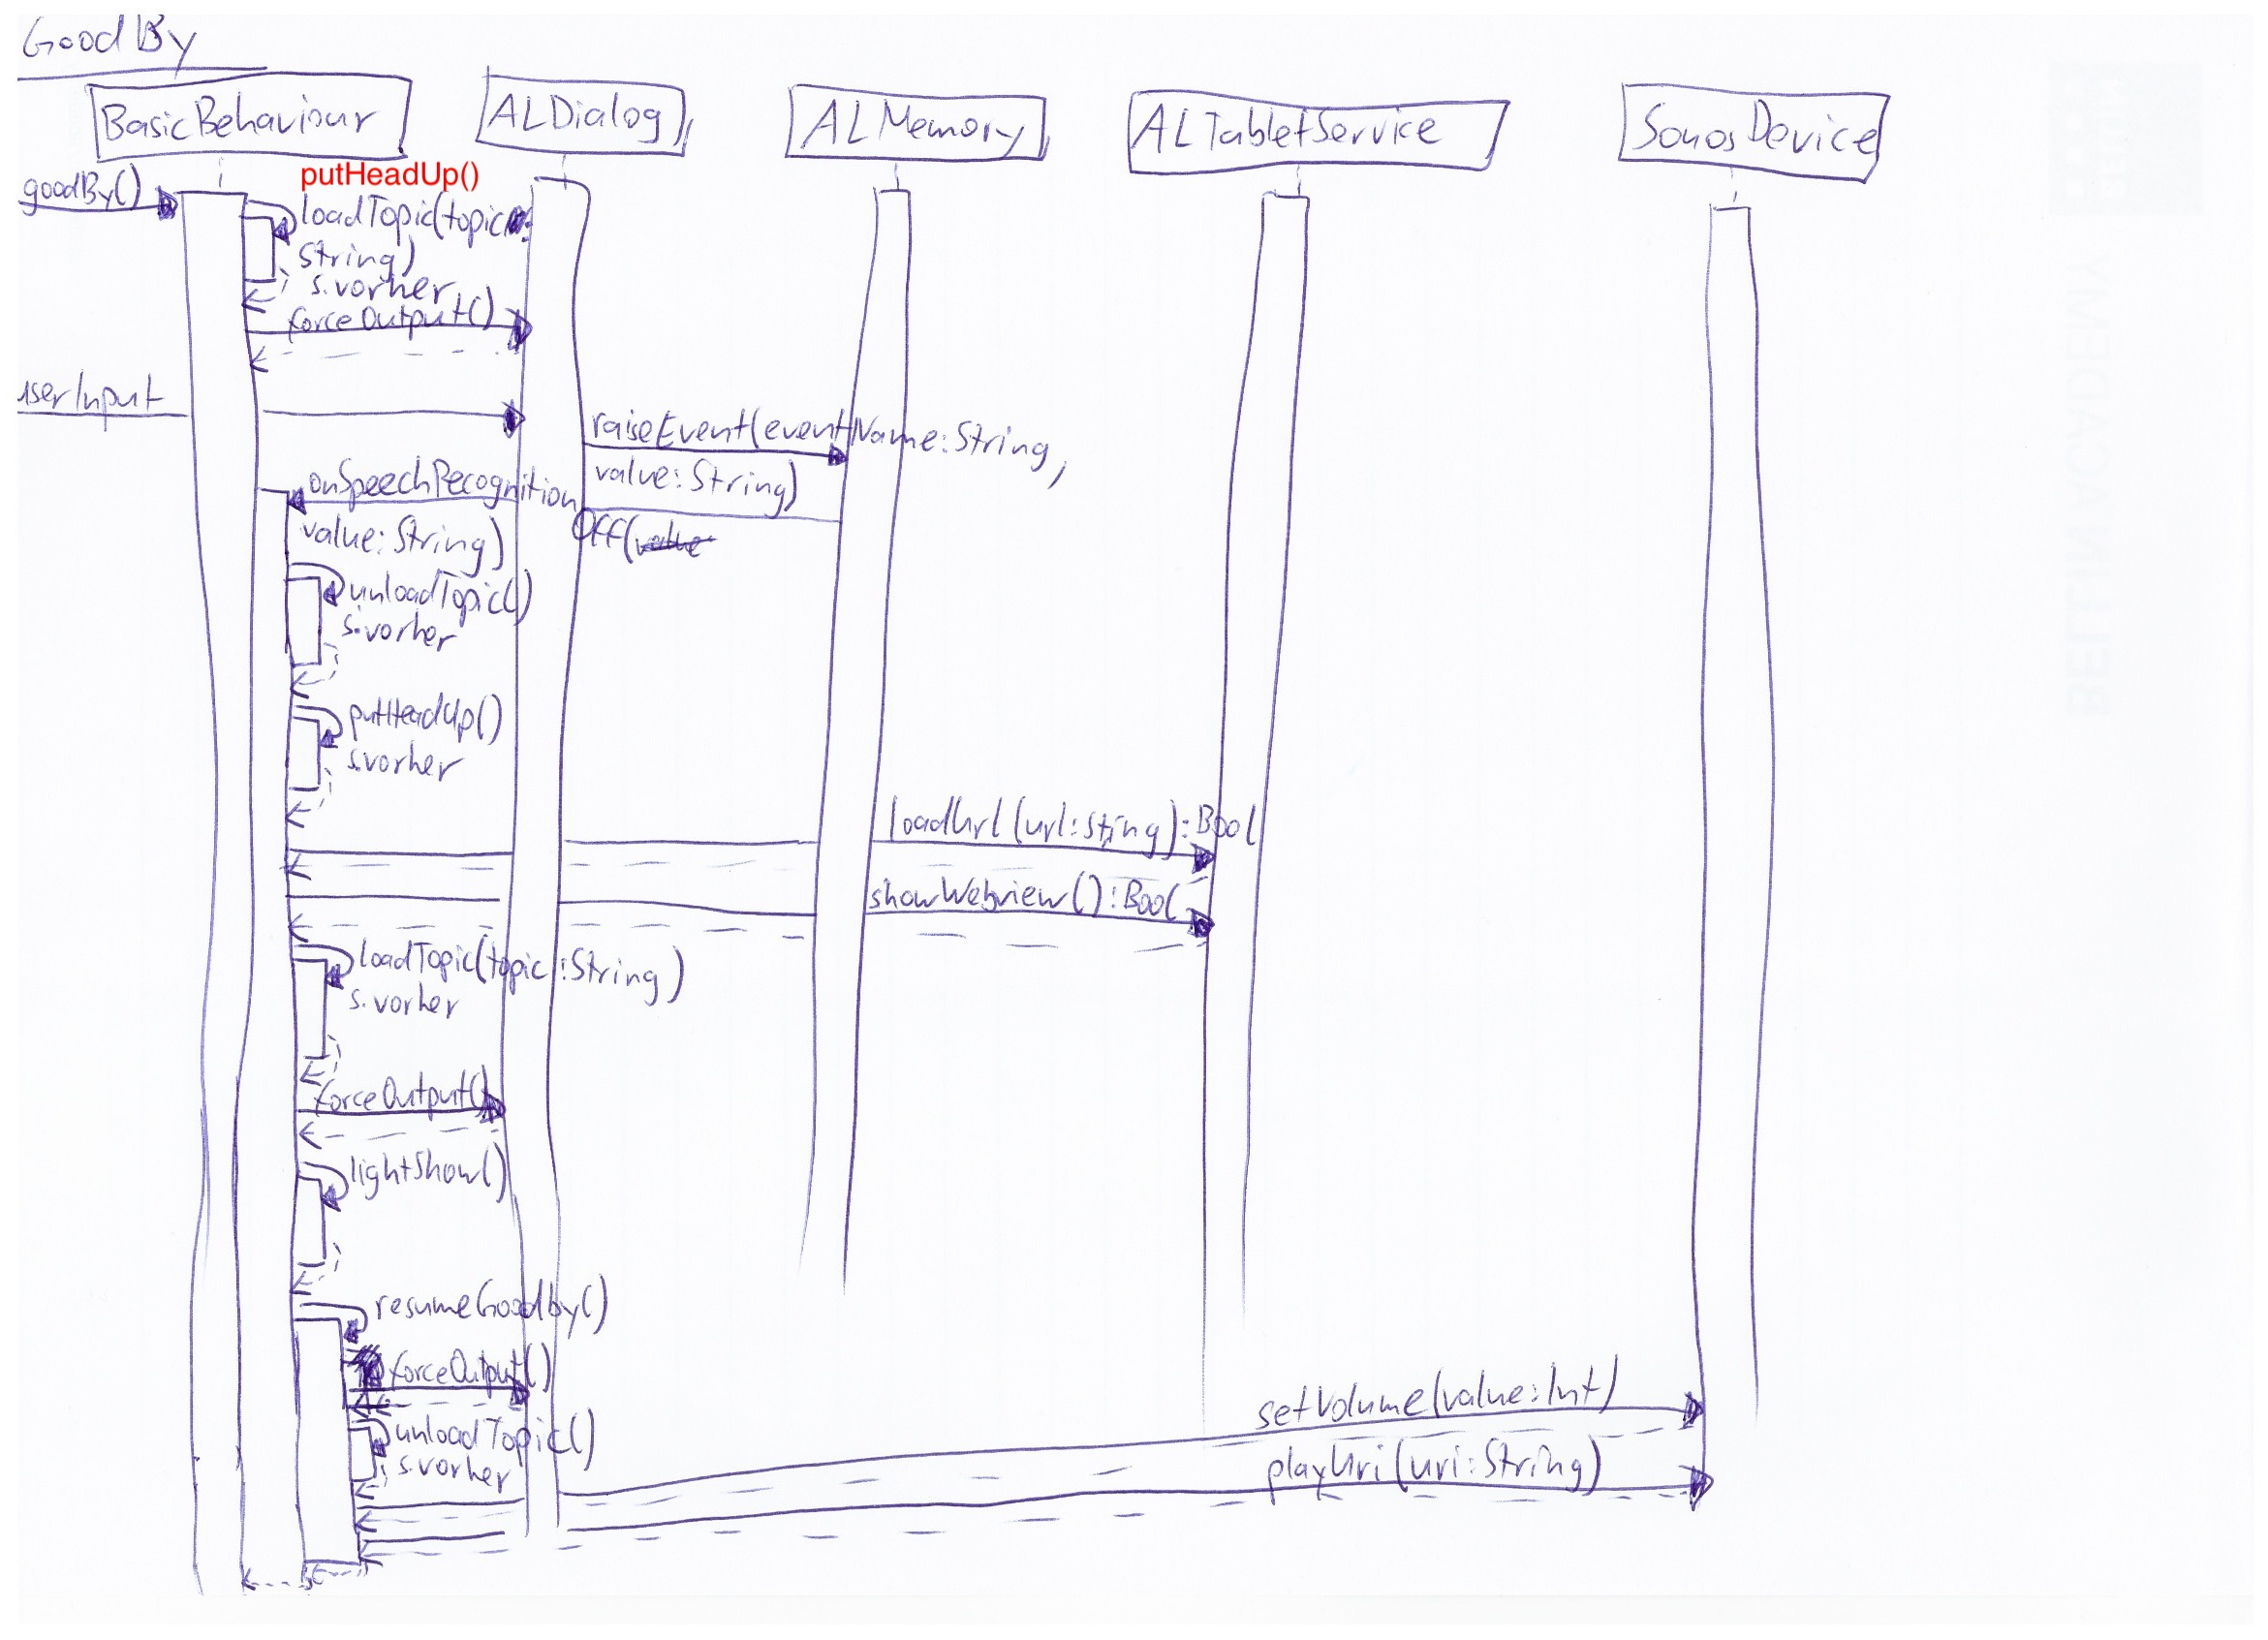
\includegraphics[width=\textwidth]{Scan_8.jpeg}
	\caption{Sequenzdiagramm - Abschlussszene}
	\label{fig:sqd:goodby}
\end{figure}

\section{Klassendiagramme}


\section{Besonderheiten bei der Programmierung}
\begin{itemize}
	\item Dialogdateien müssen immer in einem Verzeichnis auf dem Roboter liegen! Für diese Anwendung wurde das Home-Verzeichnis (/home/nao) gewählt
	\item Nach dem Hochfahren des Roboters ist die direkte Ausgabe eines \lstinline|proposals| nicht möglich. Es muss zuerst eine Nutzereingabe (reale Nutzereingabe oder programmatische Nutzereingabe macht keinen Unterschied) erfolgen
\end{itemize}


\end{document}














